\documentclass[11pt,a4paper]{article}

\usepackage[utf8]{inputenc}
\usepackage[export]{adjustbox}
\usepackage[spanish]{babel}
\usepackage{float}
\usepackage{amsmath}
\usepackage{amsfonts}
\usepackage{amssymb}
\usepackage{makeidx}
\usepackage{graphicx}
\usepackage{lmodern}
\usepackage{kpfonts}
\usepackage{wrapfig}
\usepackage{caption}
\usepackage{subcaption}
\usepackage{booktabs}
\usepackage[nottoc,numbib]{tocbibind} %agrega la bibliografia al índice.
\usepackage[font={small,it}]{caption}
%\usepackage{fourier}
\usepackage[left=2cm,right=2cm,top=2cm,bottom=2cm,headheight=13.6pt]{geometry}
\usepackage{fancyhdr}
\usepackage{multirow}
\pagestyle{fancy}
\usepackage{mathrsfs}
\usepackage{graphicx}

%Para los gráficos en general, con las tablas...¡Ja!, arreglate.
%\begin{figure}[h!]
%\centering
%\includegraphics[width=0.7\textwidth]{} %nombre de la imagen, incluirla en el mismo directorio que este archivo.
%\caption*{} %rótulo, el asterico elimina la numeración automática. 
%\label{fig:} % para luego referirse con \ref{fig:}
%\end{figure}


\begin{document}


%%%%%%%%%%%%%%%%%%%%%%%%%%%%%%%%%%%%%%%%%%%%%%%%%%%%%%%%%%%%%%%%%%%%%%%%%%%%%%%%%%%%%%%%%%%%%%%%%%%%%%%%%%%%%%%%%%%%%%%%%%%%%%%%%
% 	TÍTULO
%%%%%%%%%%%%%%%%%%%%%%%%%%%%%%%%%%%%%%%%%%%%%%%%%%%%%%%%%%%%%%%%%%%%%%%%%%%%%%%%%%%%%%%%%%%%%%%%%%%%%%%%%%%%%%%%%%%%%%%%%%%%%%%%%

%%%%%%%%%%%%%%%%%%%%%%%%%%%%%%%%%%%%%%%%%
% University Assignment Title Page 
% LaTeX Template
% Version 1.0 (27/12/12)
%
% This template has been downloaded from:
% http://www.LaTeXTemplates.com
%
% Original author:
% WikiBooks (http://en.wikibooks.org/wiki/LaTeX/Title_Creation)
%
% License:
% CC BY-NC-SA 3.0 (http://creativecommons.org/licenses/by-nc-sa/3.0/)
% 
% Instructions for using this template:
% This title page is capable of being compiled as is. This is not useful for 
% including it in another document. To do this, you have two options: 
%
% 1) Copy/paste everything between \begin{document} and \end{document} 
% starting at \begin{titlepage} and paste this into another LaTeX file where you 
% want your title page.
% OR
% 2) Remove everything outside the \begin{titlepage} and \end{titlepage} and 
% move this file to the same directory as the LaTeX file you wish to add it to. 
% Then add \input{./title_page_1.tex} to your LaTeX file where you want your
% title page.
%
%%%%%%%%%%%%%%%%%%%%%%%%%%%%%%%%%%%%%%%%%

%----------------------------------------------------------------------------------------
%	PACKAGES AND OTHER DOCUMENT CONFIGURATIONS
%----------------------------------------------------------------------------------------

%\documentclass[12pt]{article}
%\usepackage[utf8]{inputenc}
%\usepackage[spanish]{babel}
%\begin{document}

\begin{titlepage}

\newcommand{\HRule}{\rule{\linewidth}{0.5mm}} % Defines a new command for the horizontal lines, change thickness here

\center % Center everything on the page
 
%----------------------------------------------------------------------------------------
%	HEADING SECTIONS
%----------------------------------------------------------------------------------------

\textsc{\Huge Universidad de Buenos Aires}\\[0.5cm]
\textsc{\LARGE Facultad de Ciencias Exactas y Naturales}\\[0.5cm] % Name of your university/college
\textsc{\Large Departamento de Física}\\[0.25cm] % Major heading such as course name

\begin{figure}[h]
  \centering
  
\includegraphics[scale=0.15]{Logo_DF}
  \\[0.5cm]
\end{figure}

\textsc{\large Laboratorio 3}\\[0.25cm] % Minor heading such as course title

%----------------------------------------------------------------------------------------
%	TITLE SECTION
%----------------------------------------------------------------------------------------

\HRule \\[0.4cm]
{ \huge \bfseries Transitorio y tiempo caracteristico de circuitos}\\[0.2cm] % Title of your document
\HRule \\[1cm]
 
%----------------------------------------------------------------------------------------
%	AUTHOR SECTION
%----------------------------------------------------------------------------------------

\begin{minipage}{0.4\textwidth}
\begin{center} \large
\emph{Autores:}\\
\textsc{Andreu}, Gonzalo\\ % Your name
\textsc{Malpartida}, Bryan\\ % Your name
\textsc{Pugliese}, Facundo\\ % Your name


\end{center}
\end{minipage}
~ \\[1.25cm]
%\begin{minipage}{0.4\textwidth}
%\begin{flushright} \large
%\emph{Supervisor:} \\
%Dr. James \textsc{Smith} % Supervisor's Name
%\end{flushright}
%\end{minipage}\\[4cm]

% If you don't want a supervisor, uncomment the two lines below and remove the section above
%\Large \emph{Author:}\\
%John \textsc{Smith}\\[3cm] % Your name

%----------------------------------------------------------------------------------------
%	DATE SECTION
%----------------------------------------------------------------------------------------

%\vspace{\fill}


{\large 17 de Febrero de 2016}\\[1.75cm] % Date, change the \today to a set date if you want to be precise

%----------------------------------------------------------------------------------------
%	SUMMARY SECTION: No más de 15 renglones, no te zarpes
%----------------------------------------------------------------------------------------

\begin{center}
\large{\textbf{Resumen}}

\small{El objetivo del siguiente trabajo fue caracterizar circuitos RC, RL y RCL. 

Para los dos primeros casos, los circuitos RC y RL, se buscó determinar el tiempos característico de cada uno variando los parámetros de cada sistema. Ademas de poder observar los fenómenos particulares en estos sistemas, como la carga y descarga del capacitor y la disminución de la corriente debido a la inductancia, utilizando una fuente de alimentación que emitía señales cuadradas y osciloscopio como instrumento de medición.

Por otro lado, el estudio del circuito RCL se centró en la observación de los comportamientos que tiene el mismo para distintos parámetros del sistema. Para ellos se obtenían teóricamente los valores necesarios de cada parámetro para luego $settear$ los elementos del circuito y comprobar que la evolución del sistema cumpliese el modelo teórico. Dichas observaciones se obtuvieron nuevamente utilizando una fuente de señal cuadrada y un osciloscopio.

Finalmente, el método resulto eficiente a la hora de comprobar las ecuaciones referidas al circuito RC y, en menor medida, al circuito RL. En el caso del circuito RCL, pudieron analizarse los casos extremos de comportamiento, pero no el comportamiento borde debido a lo fino del mismo.} % ACA VA EL RESUMEN

\end{center}


%----------------------------------------------------------------------------------------
%	LOGO SECTION
%----------------------------------------------------------------------------------------

%\includegraphics{Logo}\\[1cm] % Include a department/university logo - this will require the graphicx package
 
%----------------------------------------------------------------------------------------

\vfill % Fill the rest of the page with whitespace

\end{titlepage}
%\end{document} %incluir en el mismo directorio que este archivo. Equivalente a un copiar-pegar, nada de andar diciendo \begin{document} en la portada. Dejar el nombre de Caratula a la caratula.

%%%%%%%%%%%%%%%%%%%%%%%%%%%%%%%%%%%%%%%%%%%%%%%%%%%%%%%%%%%%%%%%%%%%%%%%%%%%%%%%%%%%%%%%%%%%%%%%%%%%%%%%%%%%%%%%%%%%%%%%%%%%%%%%%
% 	ENCABEZADO Y PIE DE PÁGINA.
%%%%%%%%%%%%%%%%%%%%%%%%%%%%%%%%%%%%%%%%%%%%%%%%%%%%%%%%%%%%%%%%%%%%%%%%%%%%%%%%%%%%%%%%%%%%%%%%%%%%%%%%%%%%%%%%%%%%%%%%%%%%%%%%%

\lhead{}
\chead{}
\rhead{Laboratorio 3}
\lfoot{}
\cfoot{}
\rfoot{\thepage}
\renewcommand{\headrulewidth}{1pt}
\renewcommand{\footrulewidth}{1pt}
\newcommand\Sum{\displaystyle\sum}

%%%%%%%%%%%%%%%%%%%%%%%%%%%%%%%%%%%%%%%%%%%%%%%%%%%%%%%%%%%%%%%%%%%%%%%%%%%%%%%%%%%%%%%%%%%%%%%%%%%%%%%%%%%%%%%%%%%%%%%%%%%%%%%
% Página en blanco. Cita, agradecimiento, dedicación, lo que sea pero que sea algo.
%%%%%%%%%%%%%%%%%%%%%%%%%%%%%%%%%%%%%%%%%%%%%%%%%%%%%%%%%%%%%%%%%%%%%%%%%%%%%%%%%%%%%%%%%%%%%%%%%%%%%%%%%%%%%%%%%%%%%%%%%%%%%%%


%%%%%%%%%%%%%%%%%%%%%%%%%%%%%%%%%%%%%%%%%%%%%%%%%%%%%%%%%%%%%%%%%%%%%%%%%%%%%%%%%%%%%%%%%%%%%%%%%%%%%%%%%%%%%%%%%%%%%%%%%%%%%%%%%
% 	ÍNDICE
%%%%%%%%%%%%%%%%%%%%%%%%%%%%%%%%%%%%%%%%%%%%%%%%%%%%%%%%%%%%%%%%%%%%%%%%%%%%%%%%%%%%%%%%%%%%%%%%%%%%%%%%%%%%%%%%%%%%%%%%%%%%%%%%%

%\tableofcontents %compilar dos o tres veces para verlo bien. ¡Todo un índice en unas cuantas letras!
%\newpage

%%%%%%%%%%%%%%%%%%%%%%%%%%%%%%%%%%%%%%%%%%%%%%%%%%%%%%%%%%%%%%%%%%%%%%%%%%%%%%%%%%%%%%%%%%%%%%%%%%%%%%%%%%%%%%%%%%%%%%%%%%%%%%%
% 1. RESUMEN
%%%%%%%%%%%%%%%%%%%%%%%%%%%%%%%%%%%%%%%%%%%%%%%%%%%%%%%%%%%%%%%%%%%%%%%%%%%%%%%%%%%%%%%%%%%%%%%%%%%%%%%%%%%%%%%%%%%%%%%%%%%%%%%

%\section{Resumen}
%\label{sec:resumen}



%%%%%%%%%%%%%%%%%%%%%%%%%%%%%%%%%%%%%%%%%%%%%%%%%%%%%%%%%%%%%%%%%%%%%%%%%%%%%%%%%%%%%%%%%%%%%%%%%%%%%%%%%%%%%%%%%%%%%%%%%%%%%%%
% 2. INTRODUCCIÓN: ecuaciones aquí, luego se las cita.
%%%%%%%%%%%%%%%%%%%%%%%%%%%%%%%%%%%%%%%%%%%%%%%%%%%%%%%%%%%%%%%%%%%%%%%%%%%%%%%%%%%%%%%%%%%%%%%%%%%%%%%%%%%%%%%%%%%%%%%%%%%%%%%

\section{Introducción}\label{sec:intro}
Para llevar a cabo el objetivo de caracterizar los circuitos RC, RL y RCL es necesario comprender como responden a distintos tipos de combinaciones y fuentes de voltaje. Primero, deben recordarse las leyes que dictan la caida de potencial en cada elemento; capacitor $C$, resistencia $R$ e inductancia $L$. Recordando que $\frac{dq(t)}{dt} = I(t)$

\begin{equation}{\label{leyes}}
\Delta V_C = \frac{q}{C}\quad
\Delta V_R = IR\quad
\Delta V_L = \frac{dI}{dt}
\end{equation}

Si consideramos un circuito cerrado de una unica malla compuesto por una fuente de voltaje constante $V_{0}$, una resistencia $R$ y un capacitor $C$, las leyes de Kirchoff dictan que la ecuación que rige la evolución del sistema es $V_{0} = \frac{q(t)}{C}+IR$ donde $q(t)$ es la carga eléctrica del capacitor. Entonces, si tomamos como condición inicial $q(0)=0$ la solución de la ecuación es:
   
\begin{equation}{\label{RC_carga}}
q(t)=V_{0}C(1-e^\frac{-t}{RC})
\end{equation}

Y al ser $q(t)$ una exponencial creciente se denomina a este fenómeno como la \textit{carga} del capacitor.

Ahora si, utilizando una \textit{llave ideal}, se corta la fuente $V$ a tiempo $t_{0}$ la nueva solución del sistema es de la forma:

\begin{equation}{\label{RC_descarga}}
q(t-t_{0})=V_{0}C(1-e^\frac{-t_{0}}{RC})e^\frac{-t}{RC}
\end{equation}

Entonces se define a $\tau_{RC}=RC$ \textit{tiempo característico} del circuito. Por lo tanto, si $\tau_{RC}<t_{0}$ se puede observar el efecto de \textit{descarga} del capacitor pues $q(t-t_{0})$ es una exponencial decreciente. Para la corriente $I(t) = \frac{dq(t)}{dt}$, las ecuaciones que describen su comportamiento en cada caso son:

\begin{equation}{\label{RC_carga_I}}
q(t)=\frac{V_{0}}{R}e^\frac{-t}{RC}
\end{equation}

\begin{equation}{\label{RC_descarga_I}}
q(t-t_{0}) = \frac{V_{0}}{R}(e^\frac{t_{0}}{RC}-1)e^\frac{-t}{RC}
\end{equation}

Por otro lado, si en el circuito anterior se reemplaza al capacitor $C$ por una inductancia $L$, la noción de carga desaparece y queda la de corriente $I(t) = \frac{dq(t)}{dt}$ en una ecuación diferencial de la forma $V_{0} = L.\frac{dI(t)}{dt}+R.I(t)$. La solución para el caso de $V= V_0$ es muy similar a la anterior:

\begin{equation}{\label{RL_carga_I}}
I(t)=\frac{V_0}{R}(1-e^\frac{-Rt}{L})
\end{equation}

\begin{equation}{\label{RL_carga}}
\dfrac{dI(t)}{dt}=\frac{V_{0}}{L}e^\frac{-Rt}{L}
\end{equation}

En este caso, el papel del \textit{tiempo característico} lo juega $\tau_{RL}=\frac{L}{R}$ y puede verse que la corriente $I$ \textit{aumenta} hasta alcanzar su valor ideal (el valor de la corriente en un circuito sin inductancia).

Cuando se corta la fuente $V$ a tiempo $t_{0}$ tenemos el caso en que la corriente $I$ \textit{disminuye} hasta volverse nula. En esta situación, la solución del sistema es: 

\begin{equation}{\label{RL_descarga_I}}
I(t-t_0)= \frac{V_{0}}{R}(1-e^\frac{-Rt_0}{L})e^\frac{-Rt}{L}
\end{equation}

\begin{equation}{\label{RL_descarga}}
\dfrac{dI(t-t_{0})}{dt}=-\frac{V_{0}}{L}(e^\frac{Rt_{0}}{L}-1)e^\frac{-tR}{L}
\end{equation}


Un circuito más complicado puede generarse combinando los dos anteriores; una fuente de voltaje constante $V_0$, una resistencia $R$, un capacitor $C$ y una inductancia $L$. En este caso, la ecuación diferencial que rige la dependencia temporal de la carga $q(t)$ resulta:

\begin{equation}{\label{ec_RCL}}
\frac{d^2q(t)}{dt^2}L+\frac{dq(t)}{dt}R+\frac{q(t)}{C} = V_0
\end{equation}

Cuyo polinomio característico resulta $\lambda^2.L+\lambda.R+\frac{1}{C} = 0$ cuyas raíces son $\lambda_{1,2} = -\frac{R}{2L} \pm \sqrt{(\frac{R}{2L})^2-\frac{1}{LC}}$ donde $\omega_o^2 = \frac{1}{LC}>0$ de denomina \textit{frecuencia natural} del circuito. Esta frecuencia $\omega_o^2 = \frac{1}{LC}$ es la frecuencia de oscilinación del circuito de en el caso en que no existe componente disipativo ($R=0$). Dependiendo del valor del discriminante $\omega^2 = \beta^2-\omega_o^2$ donde $\beta = \frac{R}{2L}>0$ las soluciones del polinomio característico serán reales, real doble o complejas no reales y la función $q(t)$ tendrá un comportamiento sobreamortiguado, subamortiguado o amortiguado, respectivamente. 

Para el caso $\beta < \omega_o$ resulta $\omega^2 < 0$ y por lo tanto las raíces del polinomio característico son complejas y distintas. Esto conlleva a una solución de la forma:

\begin{equation}{\label{amort}}
q(t) = a.e^{-\beta t}.cos(|\omega|(t+\phi)) + V_0C
\end{equation}

donde $a$ y $\phi$ se obtienen a través de las condiciones iniciales del sistema y $|\omega| = \sqrt{\omega_o^2-\beta^2}$. Este es el caso del \textit{oscilador amortiguado}.

Para el caso $\beta = \omega_o$ se tiene $\omega^2 = 0$ y la raíz del polinomio característica resulta doble y única. Esto conlleva a una solución de la forma:

\begin{equation}{\label{sub}}
q(t) = e^{-\beta t}(A+B.t) + V_0C
\end{equation}

donde A y B nuevamente se obtienen a través de las condiciones iniciales del sistema. Este es el caso límite conocido como \textit{oscilador subamortiguado}.

Finalmente, para el caso $\beta > \omega_o$ es $\omega^2>0$ y las raíces del polinomio característico son reales y distintas. Esto conlleva a una solución exponencial de la forma:

\begin{equation}{\label{sobre}}
q(t) = e^{-\beta t}[C.cosh(\omega t)+D.sinh(\omega t)]
\end{equation}

donde C y D se obtienen a través de las condiciones iniciales del sistema. Este caso corresponde al \textit{oscilador sobreamortiguado}, dado que al ser una combinación lineal de exponenciales decrecientes ($\beta > \omega > 0$) nunca puede completarse una oscilación. 

Si, como en el caso de los circuitos RC y RL, se utiliza una señal cuadrada para simular una \textit{llave ideal}, dado que todos los comportamientos cumplen $q(t\rightarrow\infty) = 0$, los períodos donde $V = 0$ resultan en una solución $q(t) = 0$ pues tanto las condiciones iniciales como la inhomogeneidad de la ecuación diferencial son nulas. Cuando la señal vuelve a adquirir el valor $V = V_0$, se recuperan las soluciones anteriores. Sin embargo, para esto se requiere una frecuencia de la señal cuadrada $\frac{\tau_f}{2} > \beta$ para asegurarse de que la carga $q(t)$ decaiga lo suficiente. 


%%%%%%%%%%%%%%%%%%%%%%%%%%%%%%%%%%%%%%%%%%%%%%%%%%%%%%%%%%%%%%%%%%%%%%%%%%%%%%%%%%%%%%%%%%%%%%%%%%%%%%%%%%%%%%%%%%%%%%%%%%%%%%%
% 3. DISPOSITIVO EXPERIMENTAL: armado del modelo, como se midio, consideraciones a la hora de medir.
%%%%%%%%%%%%%%%%%%%%%%%%%%%%%%%%%%%%%%%%%%%%%%%%%%%%%%%%%%%%%%%%%%%%%%%%%%%%%%%%%%%%%%%%%%%%%%%%%%%%%%%%%%%%%%%%%%%%%%%%%%%%%%%

\section{Desarrollo experimental}

\subsection{Circuito RC}

La primera parte del trabajo consistió en caracterizar un circuito RC. Para ello se montó un circuito utilizando un generador de funciones $\varepsilon$, una resistencia variable por décadas $R$ y un capacitor $C = (100 \pm 0,2)nF$, conectándose en serie para formar un circuito cerrado de una única malla como se ve en la \textbf{Figura \ref{fig:RC}}. 

\begin{figure}[h]
\centering
  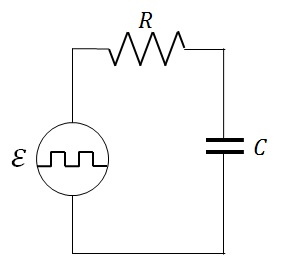
\includegraphics[scale=0.7]{Circuito-RC}
  \caption{Circuito RC con una fuente de onda cuadrada}
  \label{fig:RC}
\end{figure}

El objetivo fue medir la carga y descarga del capacitor $C$ y la corriente sobre la resistencia $R$ (que resultan proporcionales a la caida de potencial en cada elemento, respectivamente) para obtener el tiempo característico $\tau_{RC}$ del circuito determinado por (\textbf{ecucaciones de RC}).
 
Con el fin de recrear el efecto de la $llave$ $ideal$ se programó la fuente para que emitiera una señal cuadrada con un voltaje máximo $\varepsilon = (2.00 \pm 0.02)V$ y un voltaje mínimo nulo cuya frecuencia era variable. Sin embargo, esta frecuencias $f = \frac{\omega_f}{2\pi}$ debió elegirse de forma tal que la carga $q$ llegará a su máximo o mínimo (y por ende la corriente $I$ se anulase) en medio período de la señal $\frac{\tau_f}{2} = \frac{pi}{\omega_f} > \tau_{RC}$ para poder analizar todo el comportamiento.

Para medir la diferencia de tension se conectó un osciloscopio en paralelo al elemento que se quería medir, como se puede ven en la \textbf{Figura \ref{fig:RC}} donde muestra el caso de la resistencia. A su vez, el generador de funciones estaba conectado al osciloscopio para poder visualizar la forma funcional de la fuente. Se lo utilizó además como \textit{trigger externo} para poder apreciar que tanto su señal como la caida de potencial en el elemento se encontraban en fase. Y utilizando un software de recopilación de datos se pudo importar a una computadora las mediciones registradas por el osciloscopio para ser analizadas posteriormente. Este proceso se realizó para disintos valores de $R$, considerandose despreciable la resistencia aportada por $C$.

\subsection{Circuito RL}

De manera análoga, la siguiente parte del trabajo consistió en caracterizar un circuito RL. En este caso se reemplazo el capacitor $C$ por una inductancia $L = (1.000 \pm 0.002) H$. La forma del circuito se puede ver en la \textbf{Figura \ref{fig:RL}}.

\begin{figure}[h]
\centering
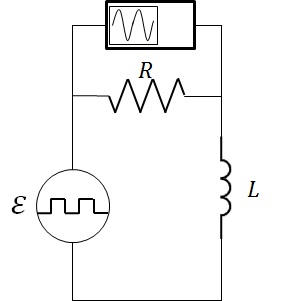
\includegraphics[scale=0.7]{Circuito-RL}
  \caption{Circuito RL con una fuente de onda cuadrada}
  \label{fig:RL}
\end{figure}

El método utilizado para obtener el tiempo característico $\tau_{RL}$, determinado por (\textbf{Ecuaciones de RL}), fue el mismo que para el circuito RC exceptuando el voltaje entregado por la fuente cuyo valor fue $\varepsilon = (8.00 \pm 0.08)V$ y la resistencia de la inductancia $R_L = (294 \pm 3) \Omega$, que en este caso no pudo ser despreciada, debió sumarse a la resistencia $R$ pues estaba en serie. Se midieron las caidas de potencial en la resistencia $R$ (proporcional a la corriente $I$) y en la inductancia $L$ (proporcional a $\frac{dI(t)}{dt}$).

Nuevamente, se buscaron frecuencias $f = \frac{\omega_f}{2\pi}$ tal que la corriente se estabilizara (llegara a un máximo o mínimo) en medio período de la señal $\frac{\tau_f}{2} = \frac{pi}{\omega_f} > \tau_{RL}$ para poder analizar todo el comportamiento.

\subsection{Circuito RCL}

Por ultimo, se buscó estudiar el comportamiento de un circuito RCL. Para ello se montó un circuito cerrado que tenia en serie la fuente programable $\varepsilon$, la resistencia variable por decadas $R$, una inductancia variable $L$ y un capacitor $C$ como muestra la \textbf{Figura \ref{fig:RCL}}.  

\begin{figure}[h]
\centering
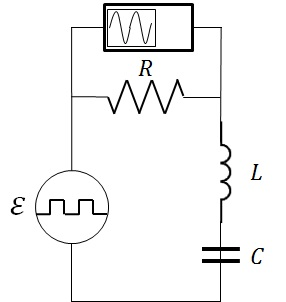
\includegraphics[scale=0.7]{Circuito-RCL}
  \caption{Circuito RCL con una fuente de onda cuadrada}
  \label{fig:RCL}
\end{figure}

Para caracterizar el circuito, la ecuación (\textbf{ecuaciones de RCL}) determina distintos \textit{comportamientos} que dependen de los parámetros que se usen.

Utilizando el método de adquisición de datos ya explicado, se midió la diferencia de potencial sobre la resistencia (que resulta proporcional a la corriente $I$). Esta diferencia de potencial era generada por una señal cuadrada de $(3.08 \pm 0.04)V$.

Por lo tanto se estudió el circuito para disintos valores de $R$,$C$ y $L$ con el fin de encontrar cada uno de estos \textit{comportamientos}. Para ello, se fijaban dos parametros y se buscaba que el tercero cumpliese las condiciones (\textbf{discriminante del polinomio que sale de la ecuacion diferencial}) que determinan cada \textit{comportamiento}.

Para cada comportamiento, como se dijo en la \textbf{Introducción}, se buscó una frecuencia $f$ tal que la corriente $I$ se anulara y, por lo tanto, se descargara el capacitor $C$ ($q=0$) en un medio período de la señal $\frac{\tau_f}{2} = \frac{pi}{\omega_f} > \beta$.


%%%%%%%%%%%%%%%%%%%%%%%%%%%%%%%%%%%%%%%%%%%%%%%%%%%%%%%%%%%%%%%%%%%%%%%%%%%%%%%%%%%%%%%%%%%%%%%%%%%%%%%%%%%%%%%%%%%%%%%%%%%%%%%%
% 4.DISCUSIÓN Y RESULTADOS: todo lo que se obtuvo y explicación. Graficos, tablas.
%%%%%%%%%%%%%%%%%%%%%%%%%%%%%%%%%%%%%%%%%%%%%%%%%%%%%%%%%%%%%%%%%%%%%%%%%%%%%%%%%%%%%%%%%%%%%%%%%%%%%%%%%%%%%%%%%%%%%%%%%%%%%%%%

\section{Resultados}
\label{sec:discusion}

\subsection{Circuito RC}
Para la primer configuracion del circuito RC, se dispuso una resistencia de $R = (3,00\pm0,02)k\Omega$, se midio la caida de potencial sobre la resistencia y mediante el analizador de datos se obtuvo un grafico que ilusta la \textbf{Figura \ref{fig:RC-CR}}

\begin{figure}[H]
\centering
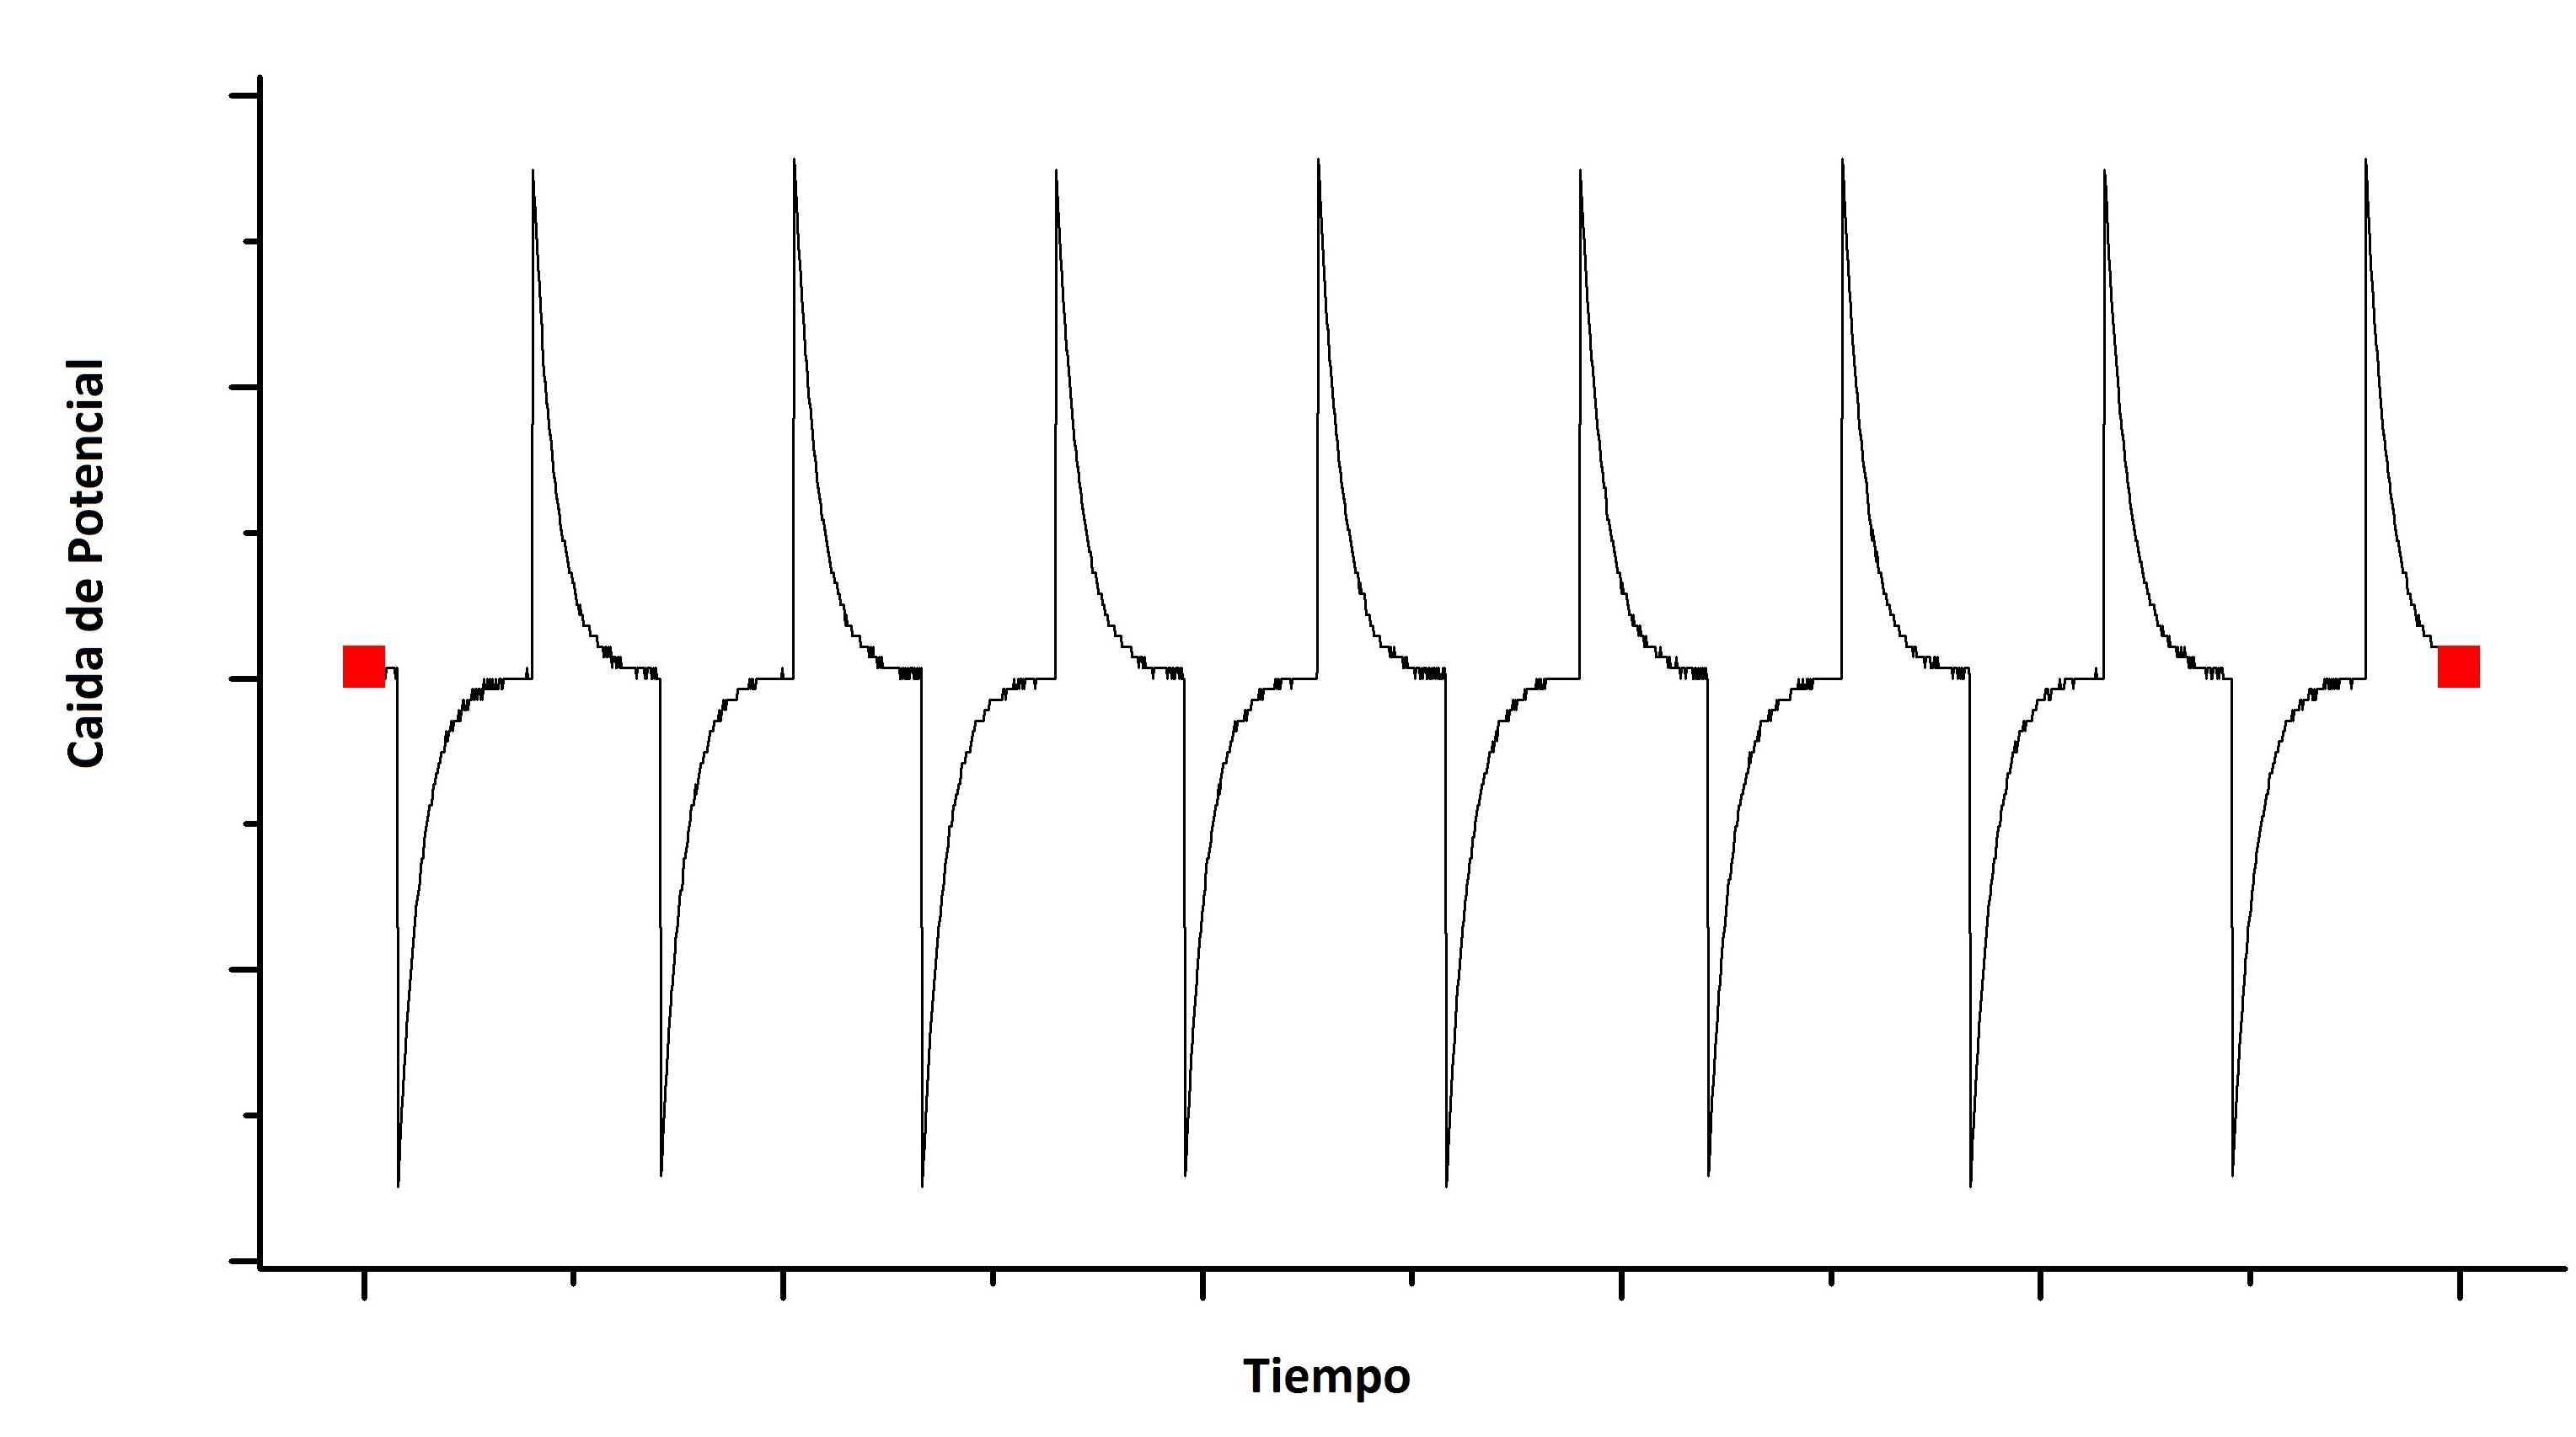
\includegraphics[scale=0.45]{RC-Caida_en_Resistencia}
  \caption{Variacion del Potencial en funcion del tiempo}
  \label{fig:RC-CR}
\end{figure}

Sabiendo que la variacion en el voltaje medida sobre la resistencia es proporcional a la corriente, se utilizaron las ecuaciones \eqref{RC_carga_I} y  \eqref{RC_descarga_I} para realizar ajustes sobre cada uno de los picos que aparecian en el grafico. Y luego se realizo un intervalo de confianza de nivel $0.95$ \textbf{(Ver apendice)} con toda la tira de datos, para obtener un valor representativo del tiempo caracteristico de este circuito, obteniendose un valor de  $\tau_{RC}=(0,315 \pm 0,004) ms$

Cuando la medicion se realizo sobre el Capacitor se obtuvo el grafico ilustrado por la \textbf{Figura \ref{fig:RC-CC}}, en el cual se utilizaron las ecuaciones \eqref{RC_carga} y \eqref{RC_descarga}; y realizandose un análisis idéntico al realizado con los valores obtenidos anteriormente, se obtuvo un $\tau_{RC}=(0,316 \pm 0,005) ms$.

\begin{figure}[H]
\centering
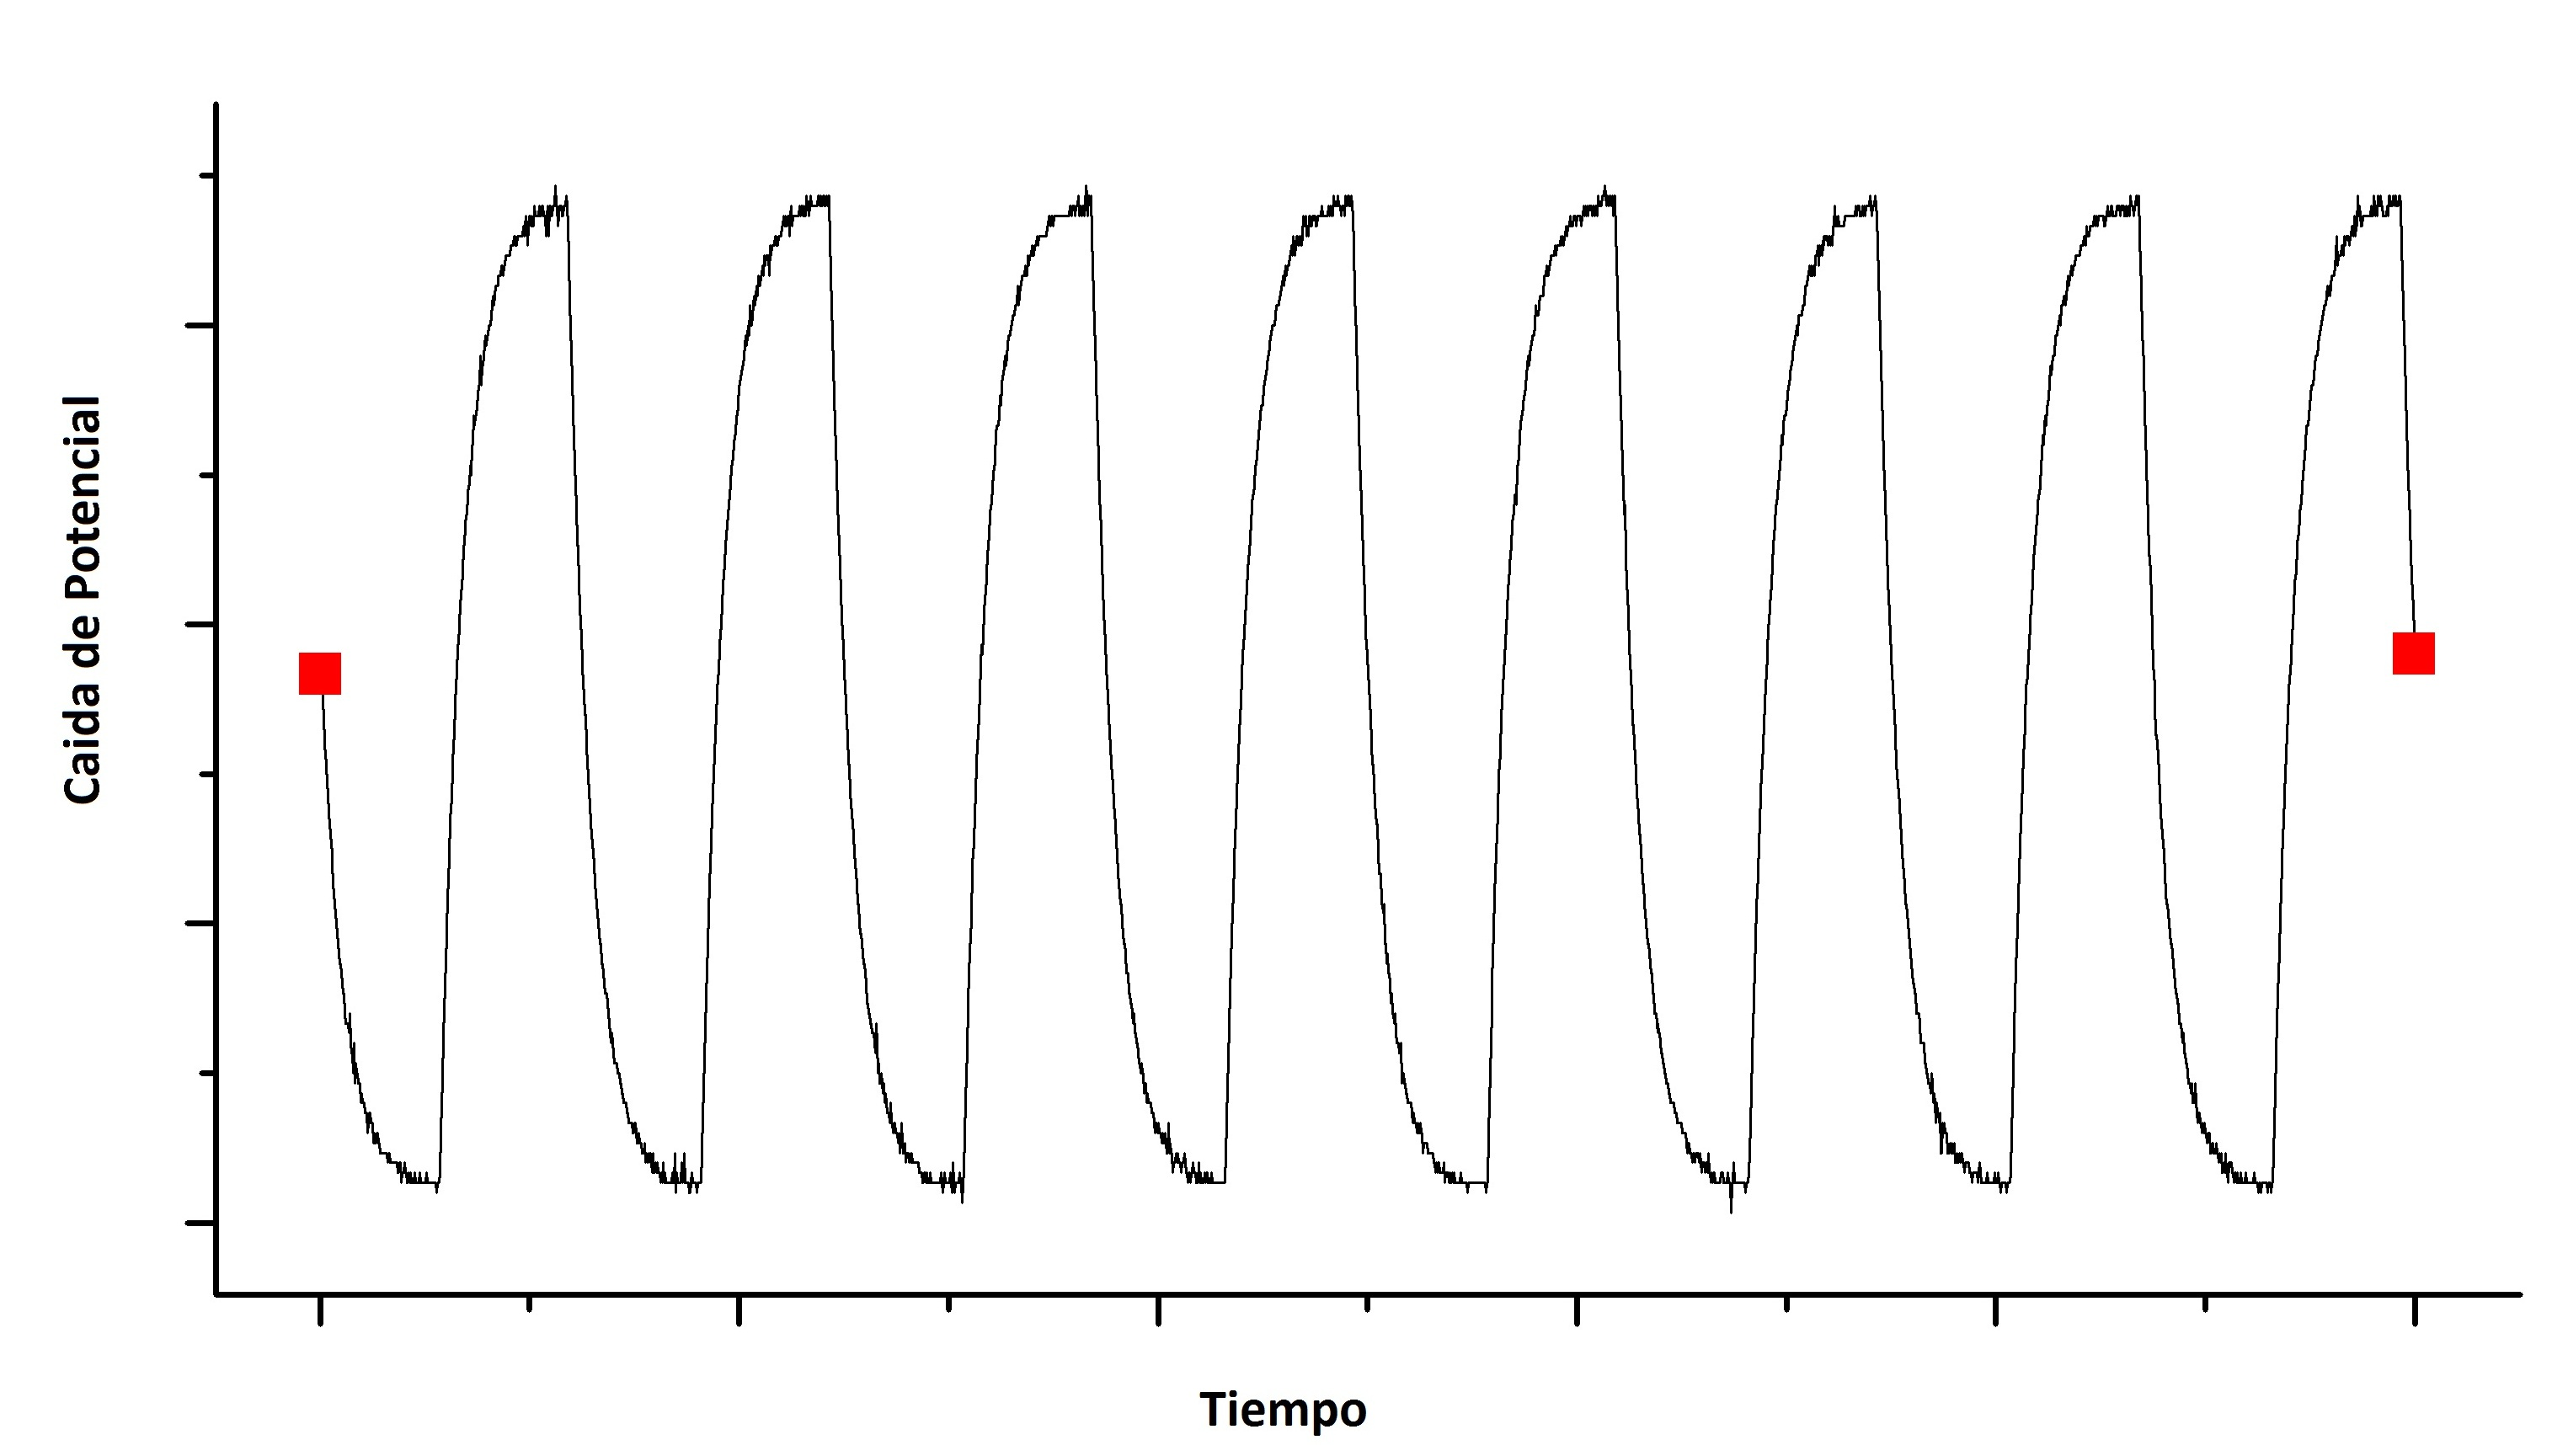
\includegraphics[scale=0.45]{RC-Caida_en_Capacitor}
  \caption{Variacion del Potencial en funcion del tiempo}
  \label{fig:RC-CC}
\end{figure}

Se puede ver que los resultados de los obtenidos de las distintas mediciones son indistigibles, ya que sus intervalos de incerteza se solapan, lo cual resulta consistente ya que el tiempo caracteristico depende intrinsecamente de la configuracion del circuito y no del lugar de la medicion.

Posteriormente se realizo el mismo analisis para configuraciones con resistencias de $(5,00\pm0,03)k\Omega, (7,00\pm0,04)k\Omega, (9,00\pm0,05)k\Omega y (11,00\pm0,05)k\Omega k\Omega$, sin variar los demas parametros y se obtuvieron los valores presentados en la \textbf{Tabla 1}, donde se puede observar lo resaltado anteriormente; para cada par de resultados correspondientes a una misma configuracion, estos son indistingibles.

\begin{center}
\begin{tabular}{||c|c|c||}
\hline
& \multicolumn{2}{c||}{\textbf{Valor}} \\ \hline
\textbf{Resistencia (k$\Omega$)} & \textbf{$\tau_{R}$ (ms)} & \textbf{$\tau_{C}$ (ms)} \\ \hline 
$(3,00\pm0,02)k\Omega$ & $0,315 \pm 0,004$ & $0,316 \pm 0,005$ \\ \hline 
$(5,00\pm0,03)k\Omega$ & $0,516\pm 0,004$ & $0,525 \pm 0,007$ \\ \hline 
$(7,00\pm0,04)k\Omega$ & $0,715\pm 0,007$ & $0,725\pm 0,006$ \\ \hline 
$(9,00\pm0,05)k\Omega$ & $0,916 \pm 0,006$ & $0,926 \pm 0,009$ \\ \hline 
$(11,00\pm0,05)k\Omega$ & $1,117\pm 0,007$ & $1,125\pm 0,005$ \\ \hline 
\end{tabular}\\[0.3cm]
 
\textit{Tabla 1: Valores obtenidos de las tiempos caracteristicos en el circuito RC}
\end{center}

Finalmente, teniendo en cuenta que segun el modelo propuesto, el tiempo caracteristico de un circuito tiene una correspondencia lineal con la resistencia se construyeron dos de gráficos que relacionan estos valores y se realizo un ajuste sobre los mismos como se puede ver en la \textbf{Figura \ref{fig:RCvsR}}.

\begin{figure}[H]

\begin{subfigure}{0.5\textwidth}
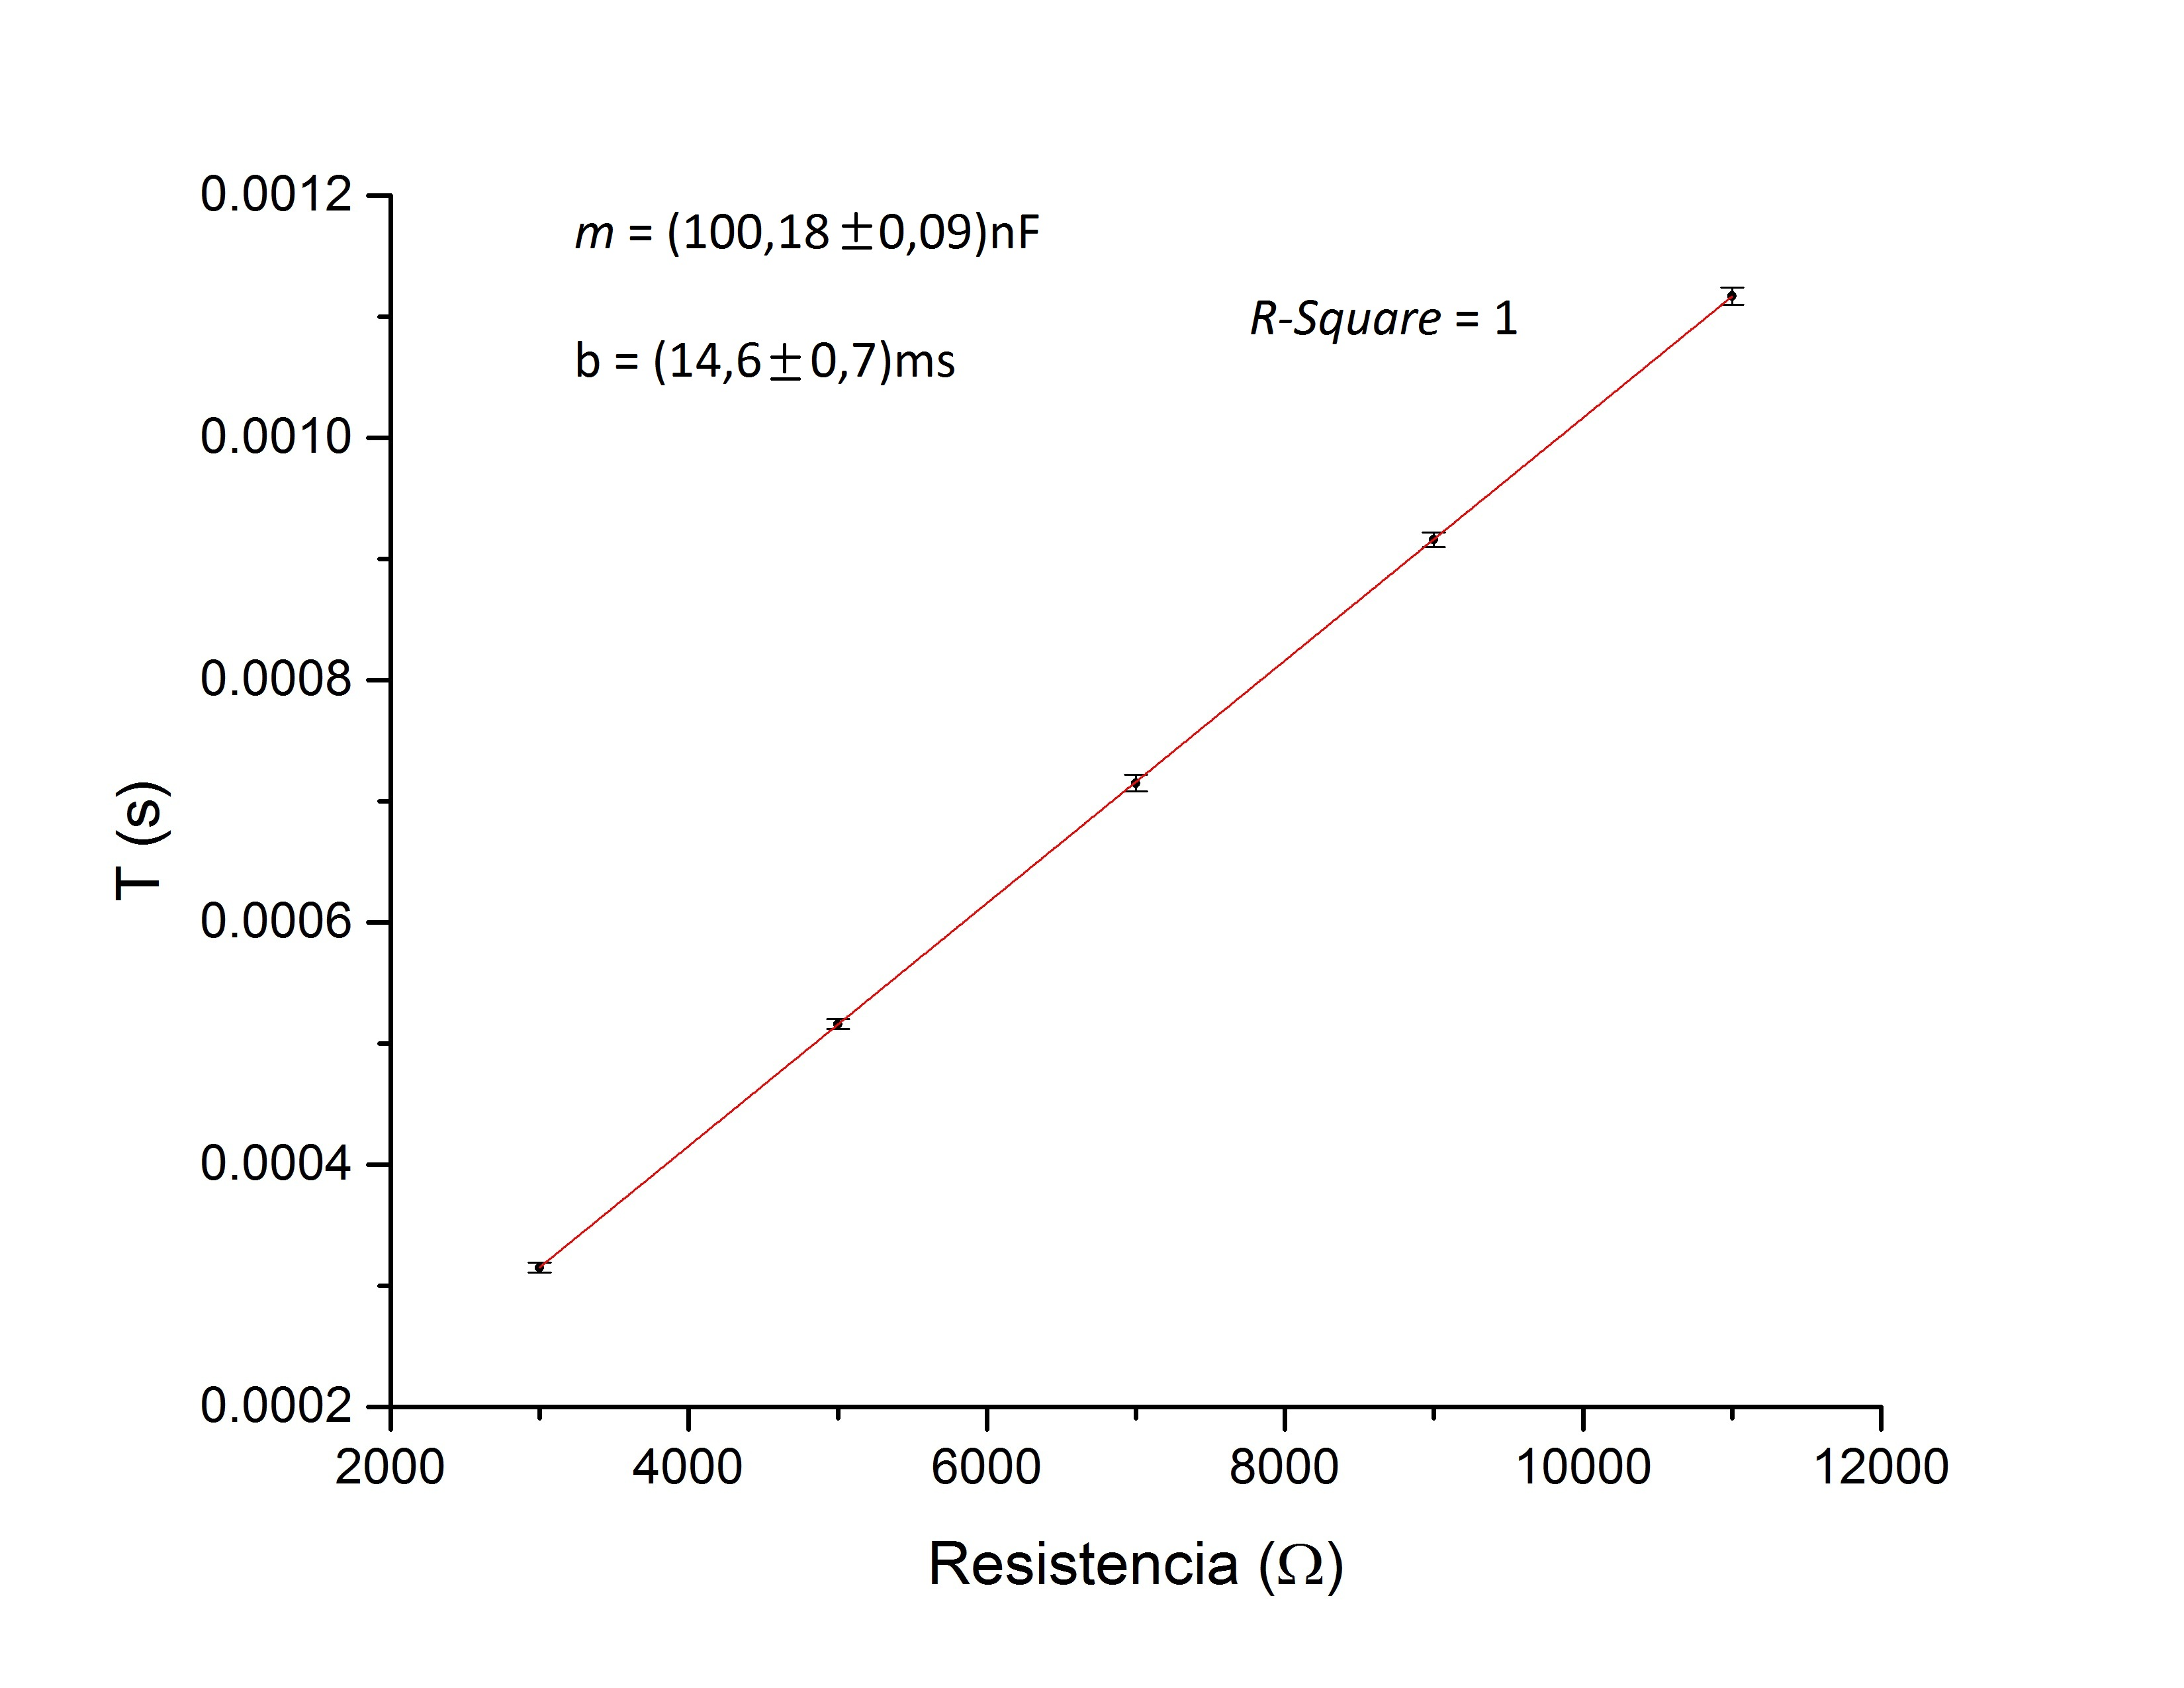
\includegraphics[scale=0.30]{Tau-RCvsR_Resistencia}
  \caption{Medicion sobre la Resistencia}
  \label{subfig:RCvsRR}
\end{subfigure}
\begin{subfigure}{0.5\textwidth}
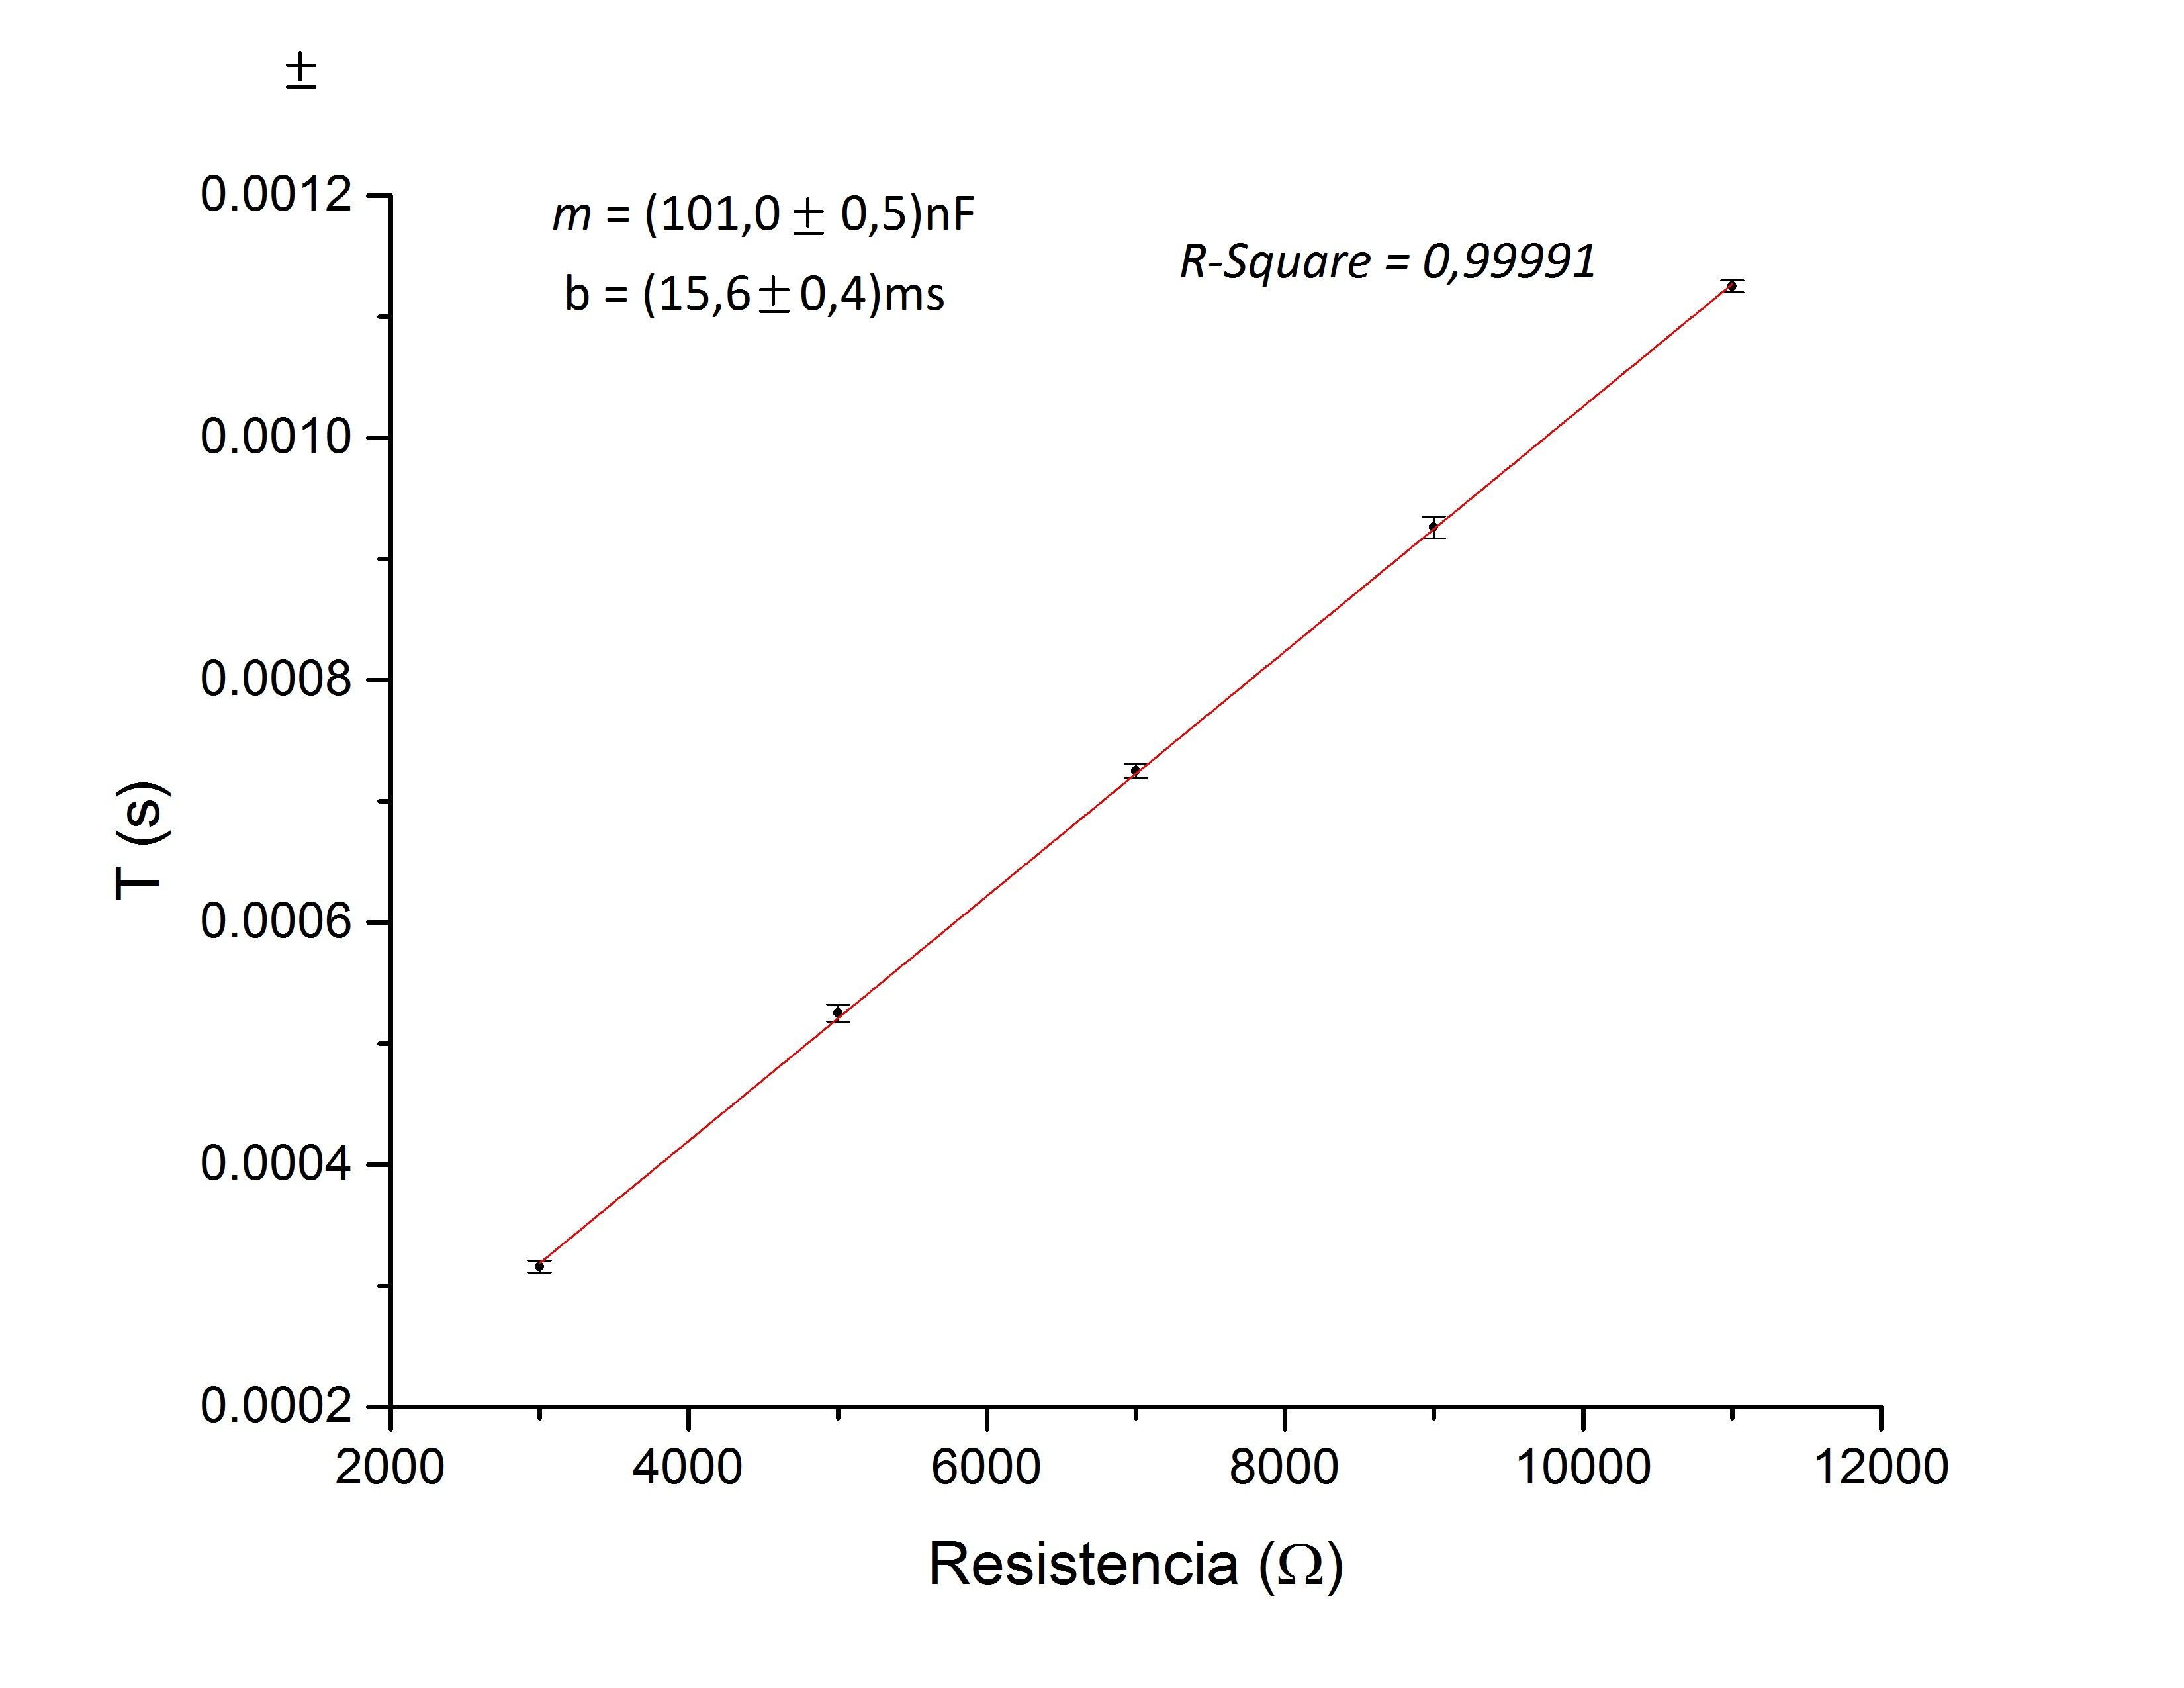
\includegraphics[scale=0.30]{Tau-RCvsR_Capacitor}
  \caption{Medicion sobre el Capacitor}
  \label{subfig:RCvsRC}
\end{subfigure}
  \caption{Variacion del tiempo caracteristico en funcion de la resistencia}
  \label{fig:RCvsR}
\end{figure}

El resultado esperado seria que la pendiente de ambos graficos sea equivalente al valor de la capacitancia $C = (100 \pm 0,2)nF$. Efectivamente para la \textbf{Figura \ref{subfig:RCvsRR}} la pendiente arroja un valor $m_{R} = (100.18 \pm 0,09)nF$ una ordenada $b_R = (14,6 \pm 0,7)\mu s$ con un coeficiente $R-Square = 1$ mientras que para la \textbf{Figura \ref{subfig:RCvsRC}} la pendiente es $m_{C} = (101 \pm 0,5)nF$ y a ordenada $b_C = (15,6 \pm 4)ms$ con un coeficiente $R-Square = 0.99991$. Los $R-square$ aseguran la bondad del ajuste y las ordenadas $b_C$, $B_R$ resultan despreciables frente a los valores $\tau_{RC}$ manejados.


\subsection{Circuito RL}

El procedimiento realizado con el circuito RL es absolutamente analogo al realizado con el RC. Se realizaron mediciones para distintas configuraciones que relevaban multiples curvas como muestra la \textbf{Figura \ref{fig:RL_C}}. En el caso de los graficos de tipo \textbf{\ref{subfig:RL_CR}}, como corresponden a las mediciones sobre la resistencia, se utilizaron las ecuaciones \eqref{RL_carga_I} y \eqref{RL_descarga_I} para realizar los ajustes, ya que la caida de potencial medida en ese lugar es proporcional a la Corriente. En cambio, para los graficos de tipo \textbf{\ref{subfig:RL_CI}}, correspondientes a las mediciones sobre la inductancia, se utilizaron las ecuaciones \eqref{RL_carga} y \eqref{RL_descarga}, ya que, en este caso, es proporcional a la derivada de la corriente.

\begin{figure}[H]

\begin{subfigure}{0.5\textwidth}
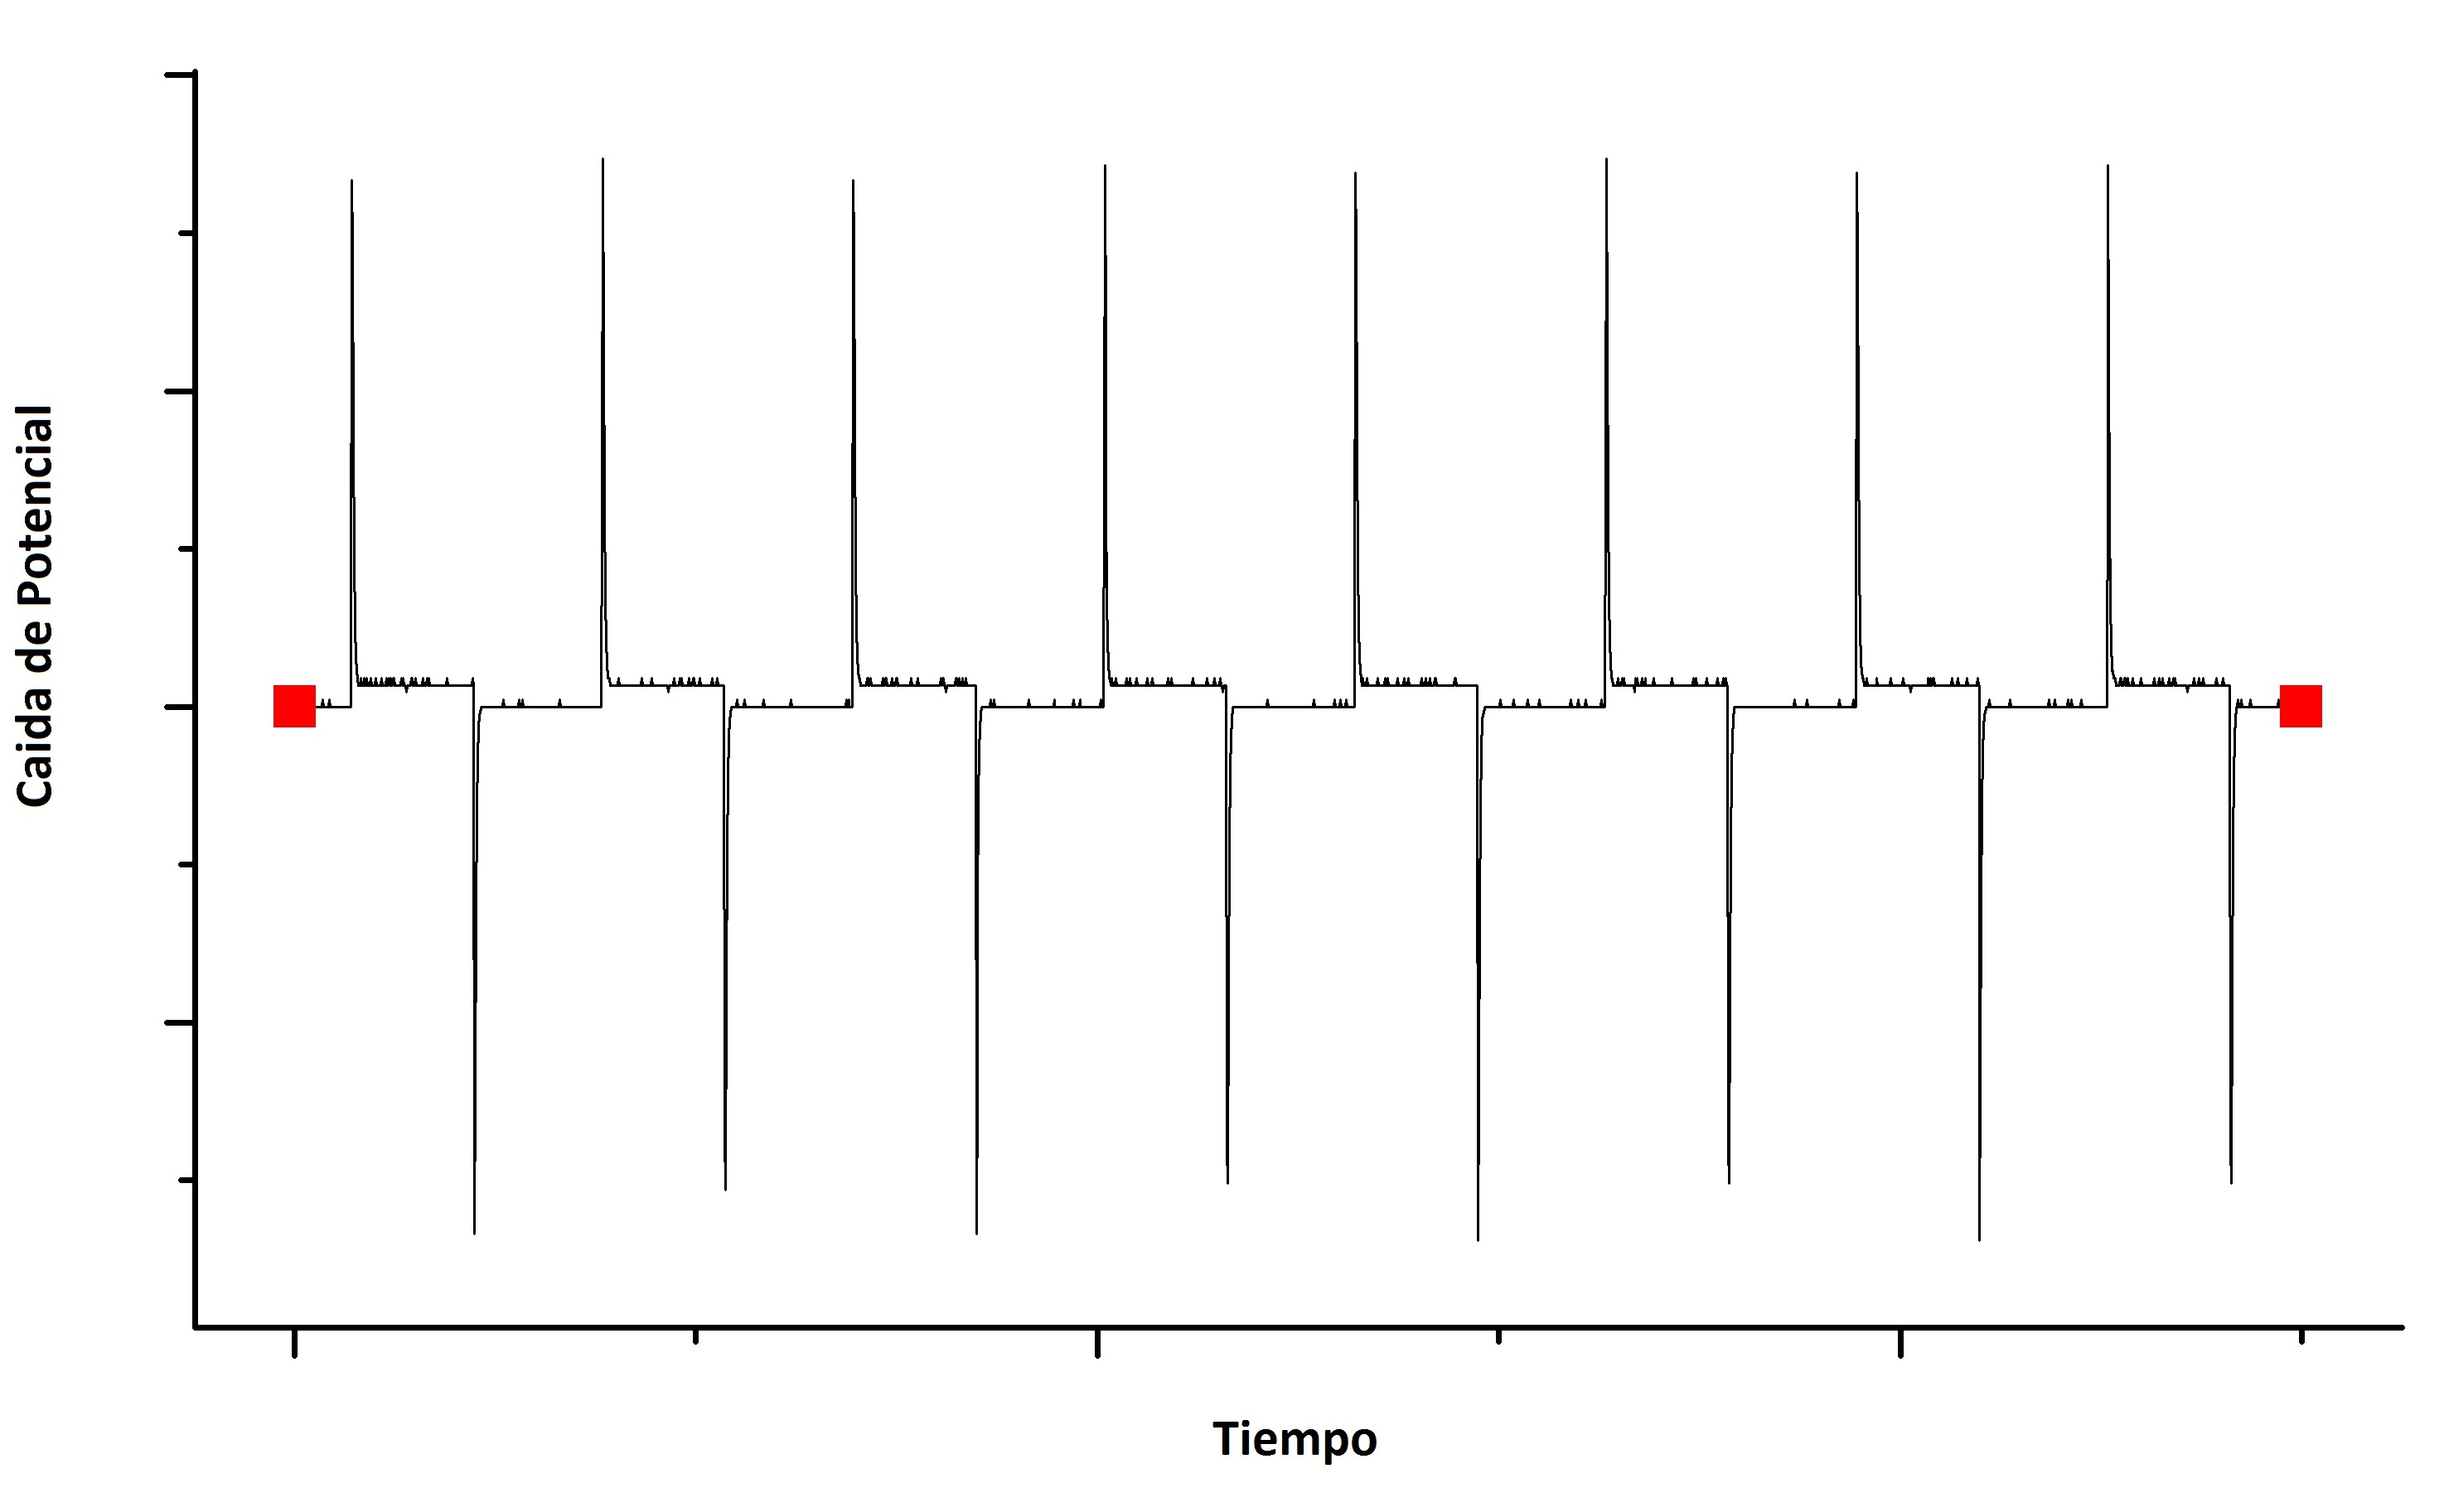
\includegraphics[scale=0.30]{RL-Caida_en_Inductancia}
  \caption{Medicion sobre la Inductancia}
  \label{subfig:RL_CI}
\end{subfigure}
\begin{subfigure}{0.5\textwidth}
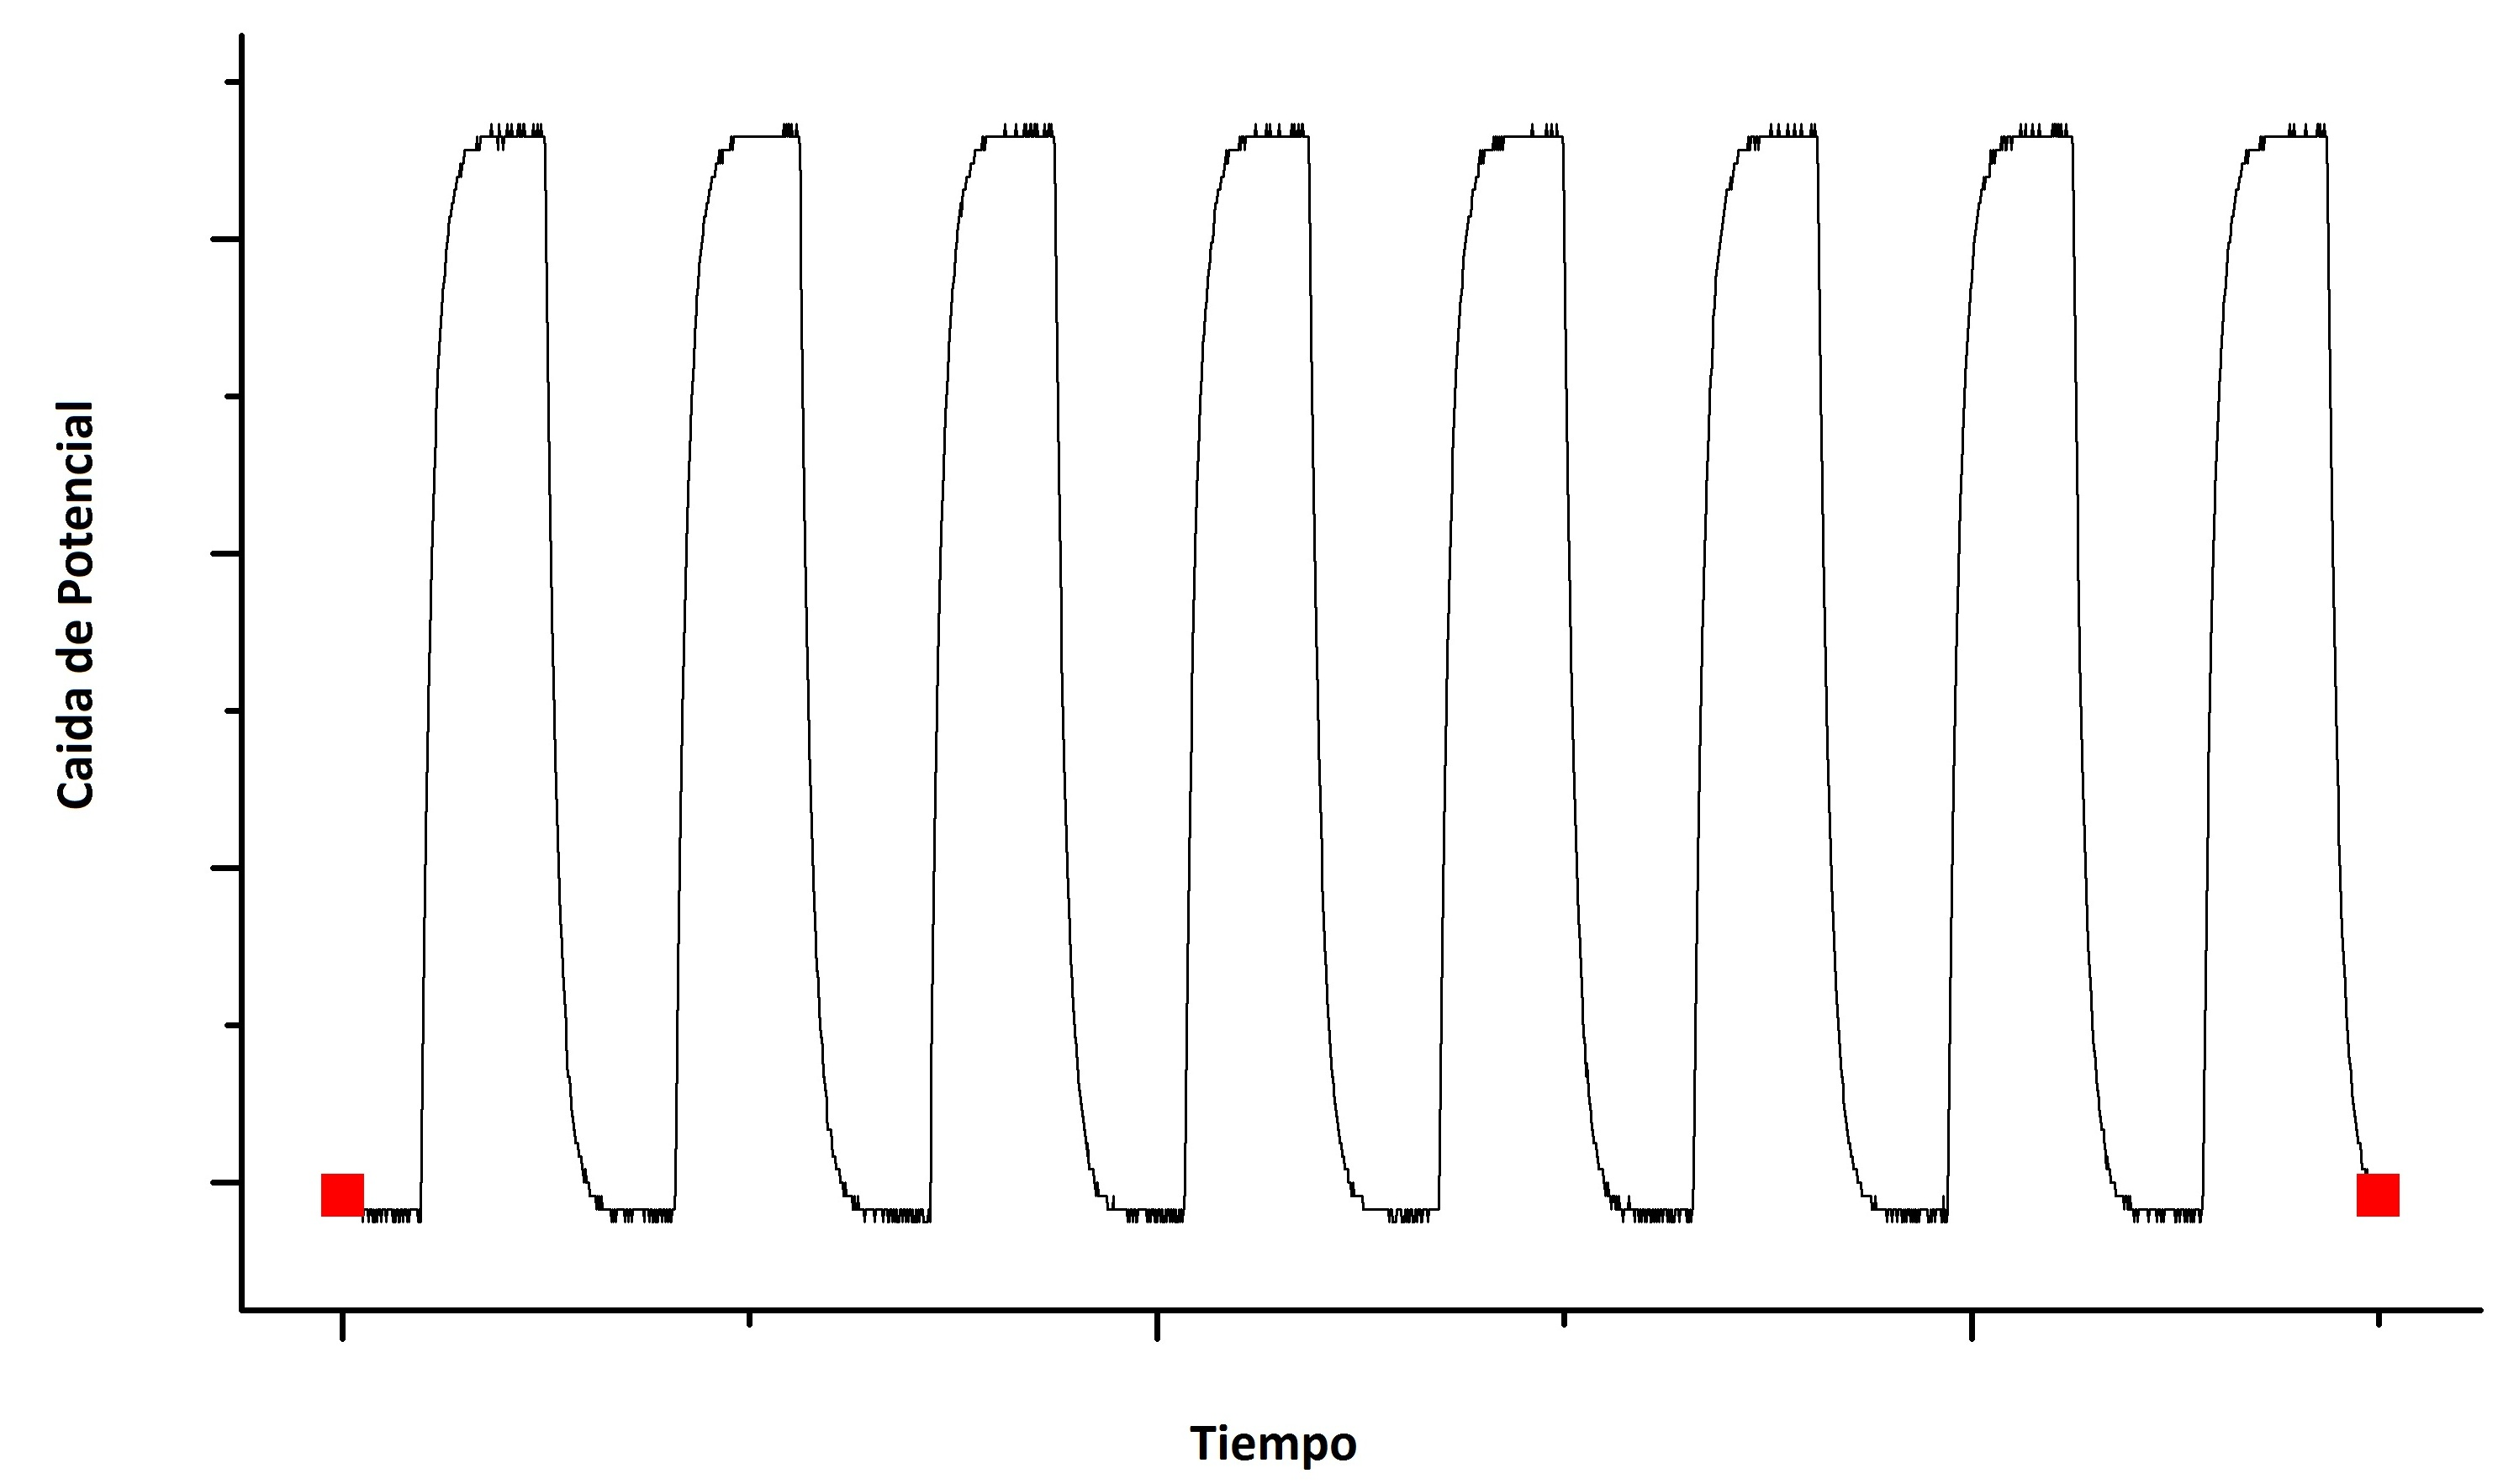
\includegraphics[scale=0.30]{RL-Caida_en_Resistencia}
  \caption{Medicion sobre la Resistencia}
  \label{subfig:RL_CR}
\end{subfigure}
  \caption{Caida del potencial en funcion del tiempo}
  \label{fig:RL_C}
\end{figure}

Posteriormente, con los resultados provistos por los ajustes, se realizo el mismo análisis, obteniendose los resultados explayados en la \textbf{Tabla 2}.

\begin{center}
\begin{tabular}{||c|c|c||}
\hline
\multicolumn{3}{||c||}{\textbf{Valor}} \\ \hline
\textbf{Posicion osciloscopio} & \textbf{Resistencia (k$\Omega$)} & \textbf{$\tau_{RL}$ (ms)}\\ \hline 
\multirow {5}{2cm}{Resistencia} & $(0.6\pm0.003)$ & $1.373 \pm 0.006$ \\ \cline {2-3}
& $(0.8\pm0.004)$ & $1.04\pm 0.01$ \\ \cline {2-3} 
& $(1\pm0.005)$ & $0.770 \pm 0.003$ \\ \cline {2-3}
& $(1.2\pm0.006)$ & $0.656 \pm 0.004$ \\ \cline {2-3}
& $(1.4\pm0.007)$ & $0.570 \pm 0.002$ \\ \hline
\multirow {5}{2cm}{Inductancia} & $3$ & $0.27 \pm 0.03$ \\ \cline {2-3}
& $(5\pm0.03)$ & $0.157 \pm 0.002$ \\ \cline {2-3}
& $(7\pm0.04)$ & $0.114 \pm 0.002$ \\ \cline {2-3}
& $(9\pm0.05)$ & $0.091 \pm 0.005$ \\ \cline {2-3} 
& $(11\pm0.05)$ & $0.071 \pm 0.008$ \\ \hline
\end{tabular}\\[0.3cm]

 \textit{Tabla 2: Valores obtenidos de los tiempos caracteristicos en el circuito RL}
\end{center}

Luego se costruyo el \textbf{grafico \ref{fig:T-RL}} que relaciona las duplas, se realizo un ajuste esperando que se respete la relacion $\tau_{RL} = L/R$ y que, ademas, se consiga un valor de $L = (1.000 \pm 0.002) H$.

\begin{figure}[H]
\centering
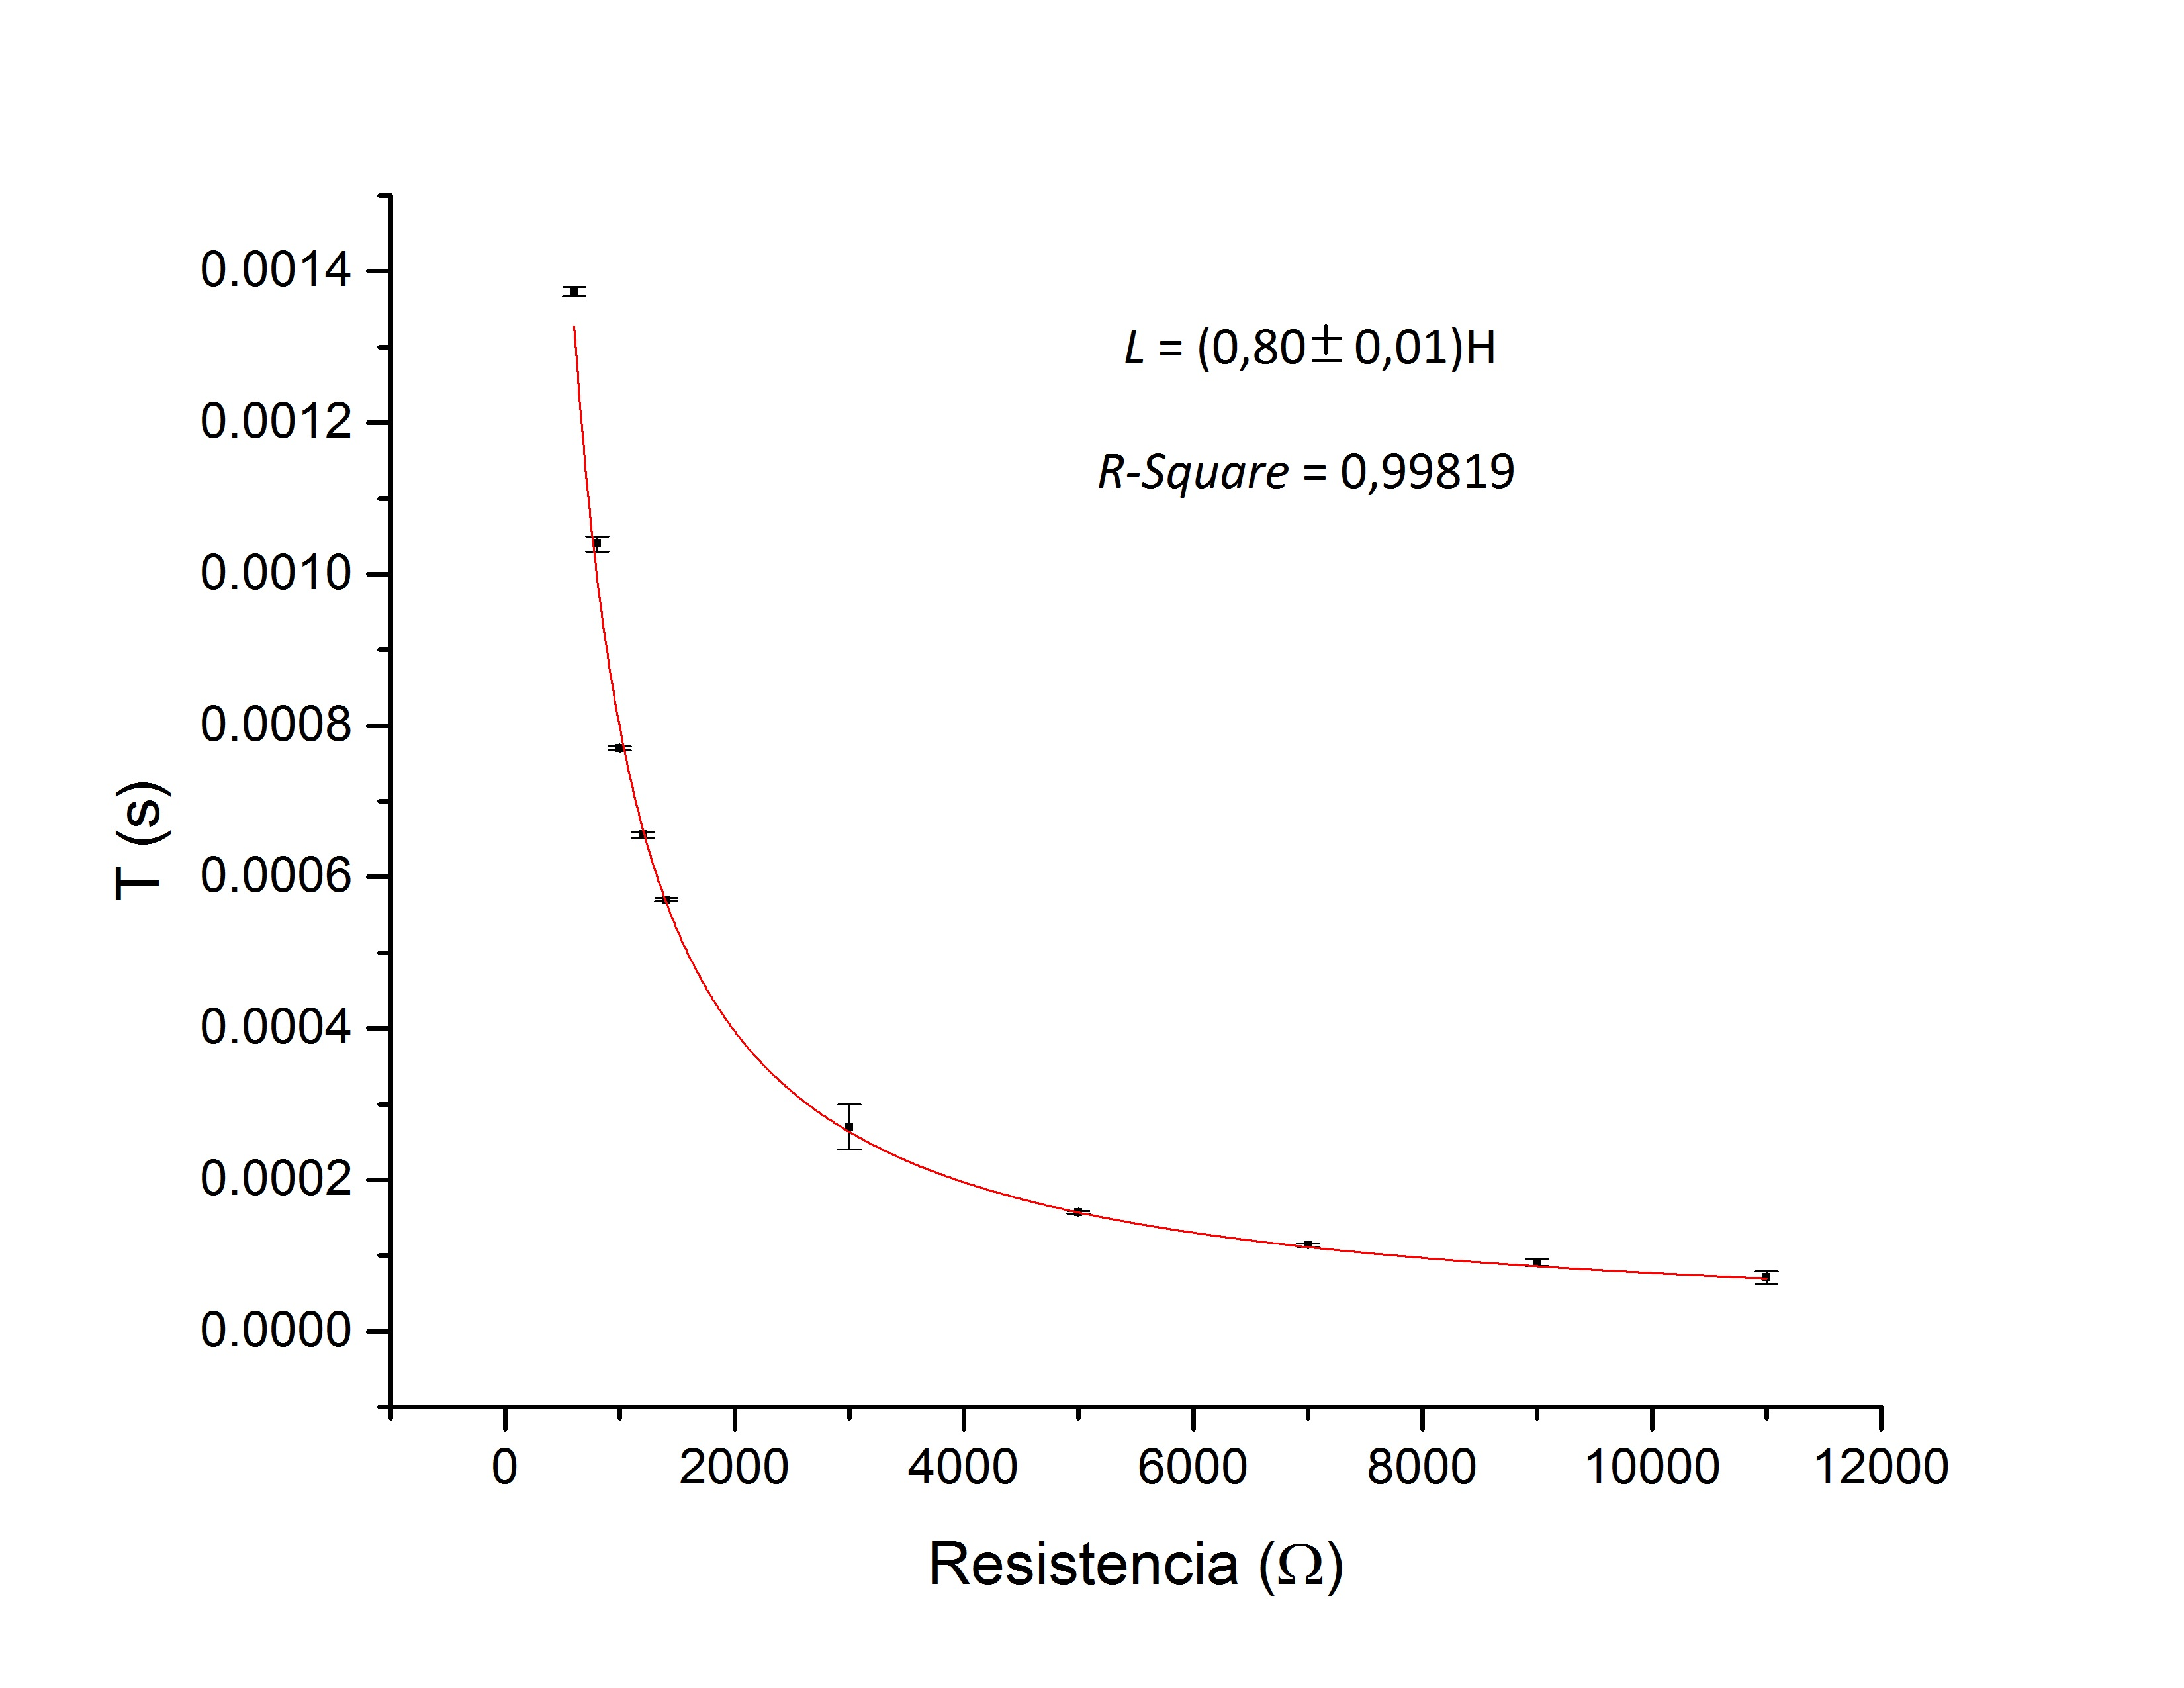
\includegraphics[scale=0.45]{TauRCvsR_Todo_en_Serie}
  \caption{Variacion del tiempo caracteristico en funcion de la resistencia}
  \label{fig:T-RL}
\end{figure}

Efectivamente, una vez realizado ese proceso, se obtiene un $R-Square = 0.99819$ que ratifica la bondad del ajuste pero, el valor de la inductancia calculado por este metodo fue $L = (0.80 \pm 0.01) H$, que es ligeramente inferior.


\subsection{Circuito RCL}

Para realizar la primer medición, se fijó una Resistencia $R= (400 \pm 4) \Omega$, una Inductancia $L = (1 \pm 0.001) H$ (la cual añadia una resistencia de $R_{L} = 296 \pm 3 \Omega$), y una capacitancia $C = (100 \pm 0.2) nF$. Bajo esos parametros se esperaba una respuesta regida por la ecuación \eqref{amort} y, efectivamente, se puede ver en la \textbf{Figura \ref{fig:RLC-A}} que el ajuste propuesto es correcto, pues arroja un $R-Square = 0.99827$. Cabe destacar, que para este tipo de circuito, no se realizó el analisis utilizado en los dos casos anteriores,por lo que se se priorizo obtener la maxima resolucion posible con el osciloscopio.

\begin{figure}[H]
\centering
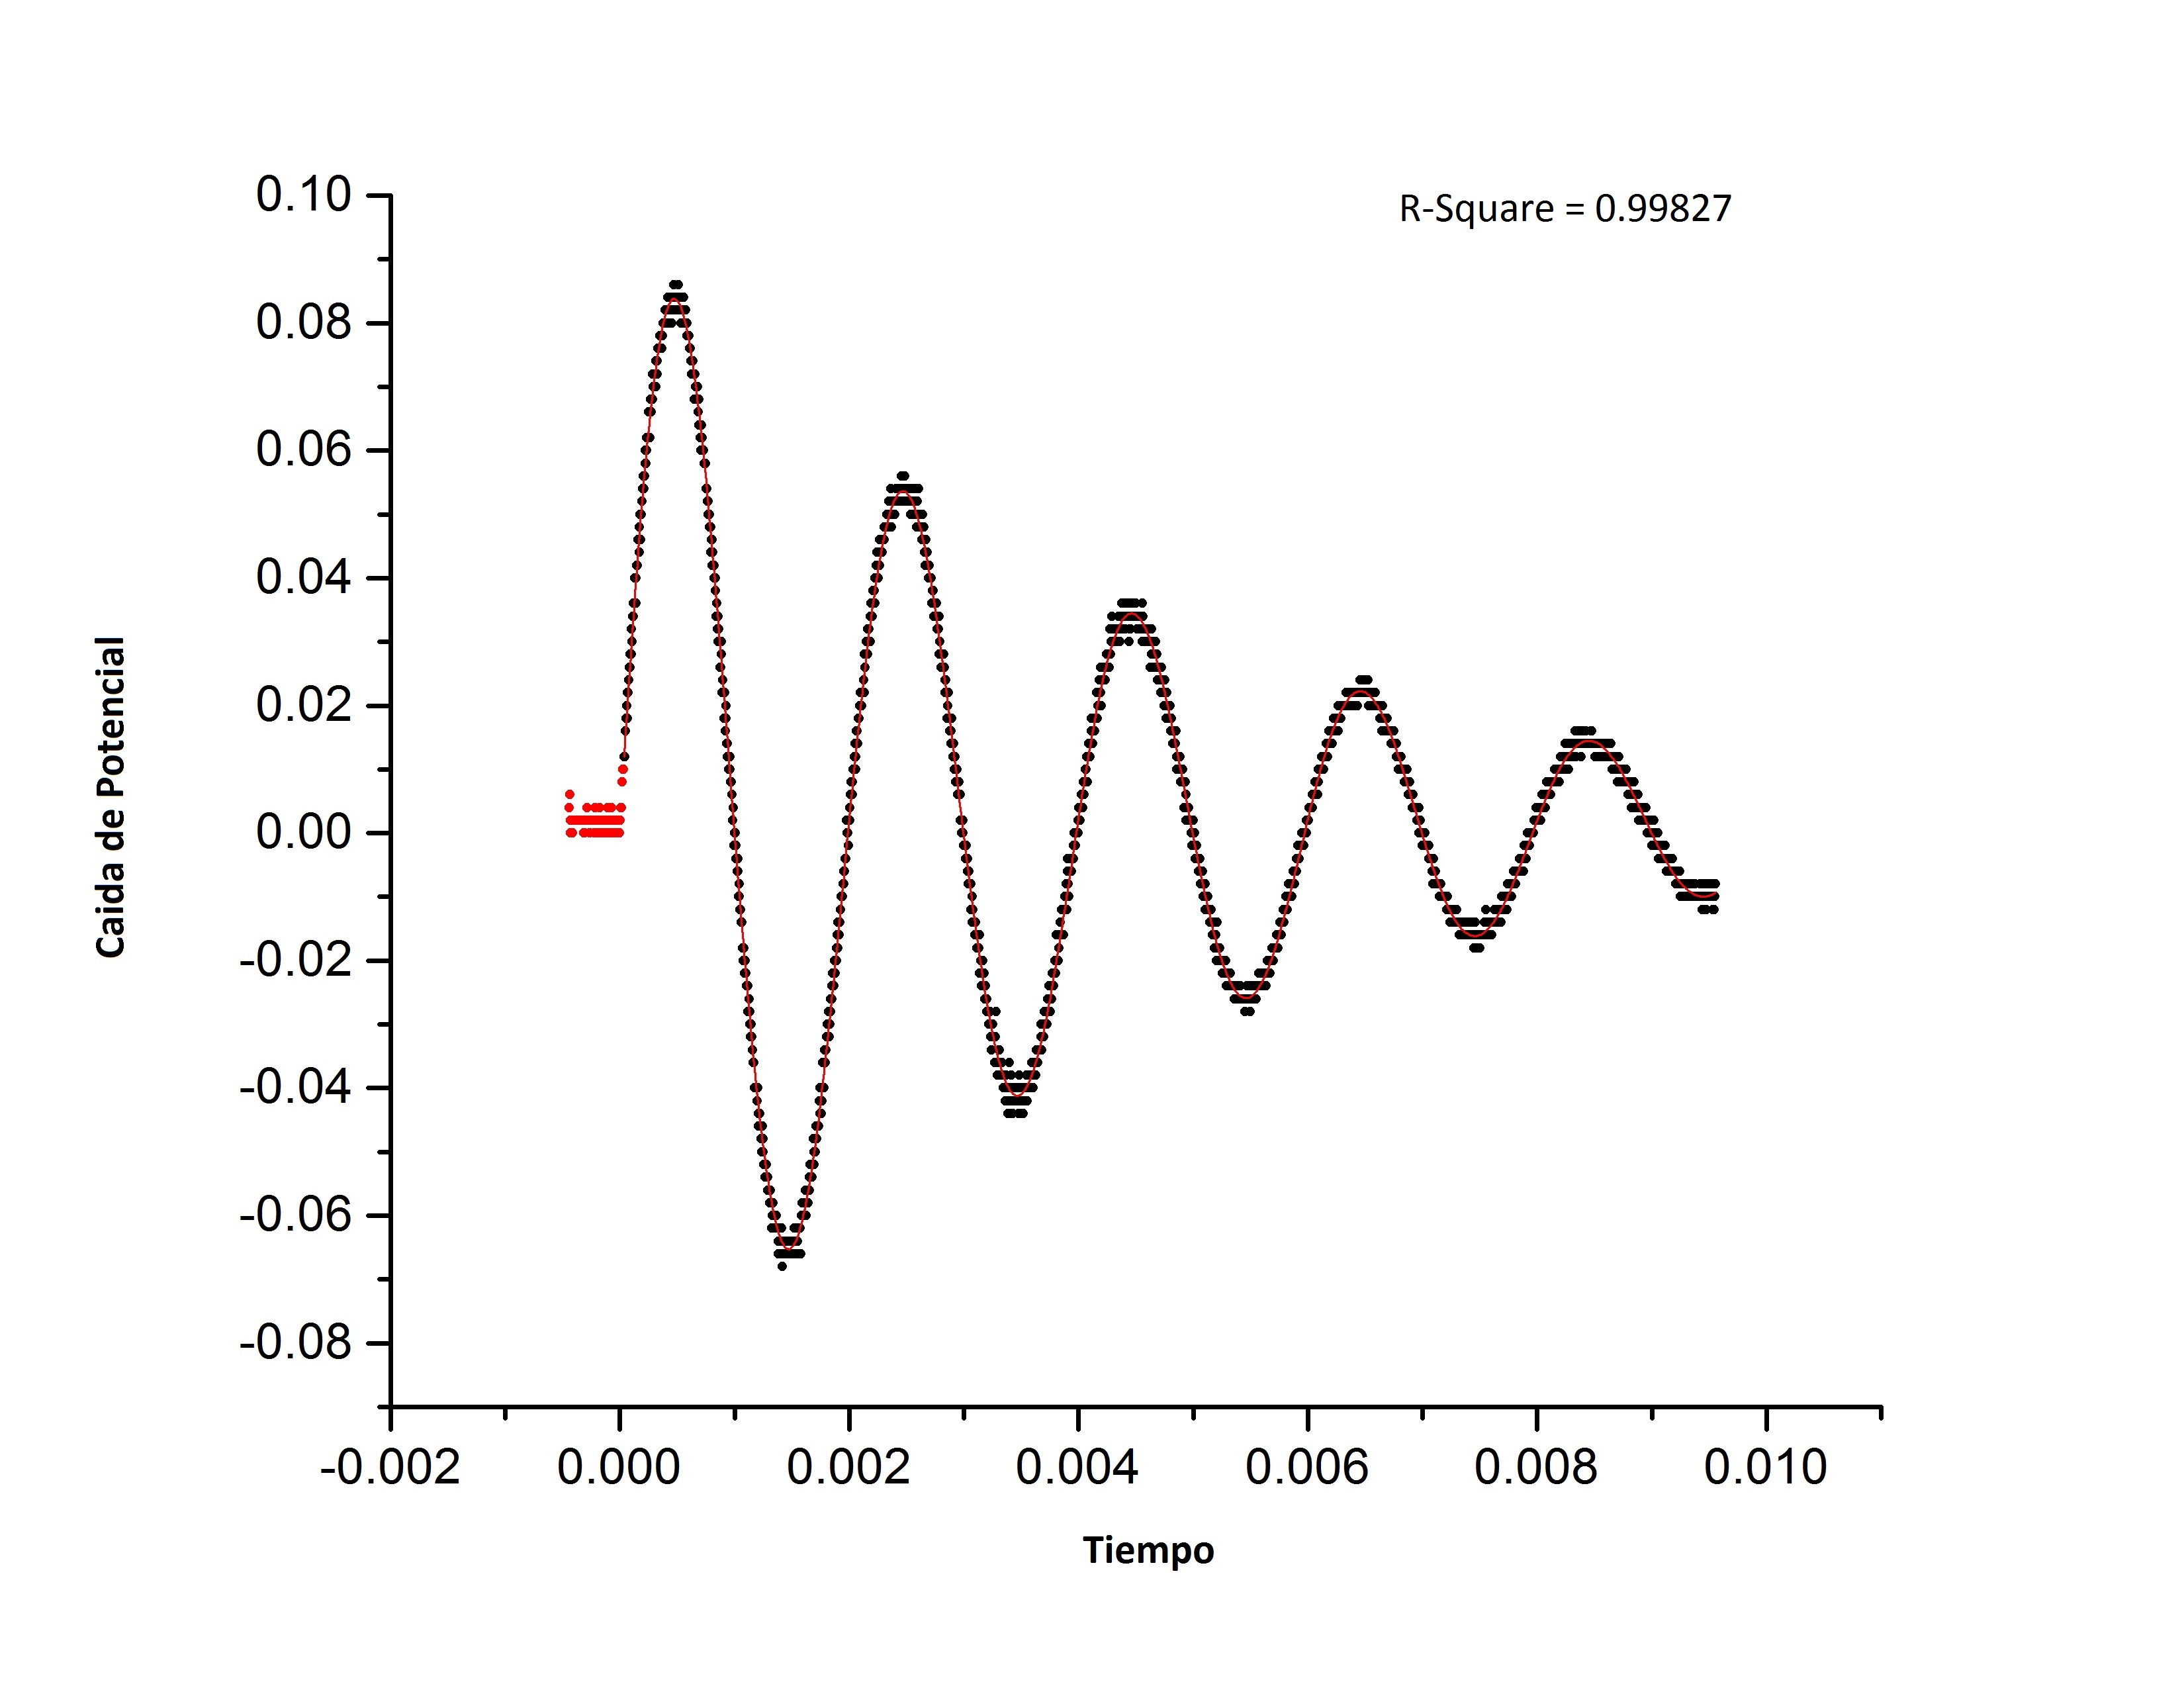
\includegraphics[scale=0.45]{RLC-Amortiguado(1H)}
  \caption{Variacion del potencial en funcion del tiempo en un circuito RLC (Oscilador amortiguado)}
  \label{fig:RLC-A}
\end{figure}

 Del ajuste se puede extraer el valor de la frecuencia de oscilacion $f_{A} = 501.3 \pm 0.7 hz$ el cual es consistente con la calculada de manera teorica, $f_{teo} = 500.2 \pm 0.6 hz$, ya que como sus intervalos de incerteza se solapan, son indistigibles.





%%%%%%%%%%%%%%%%%%%%%%%%%%%%%%%%%%%%%%%%%%%%%%%%%%%%%%%%%%%%%%%%%%%%%%%%%%%%%%%%%%%%%%%%%%%%%%%%%%%%%%%%%%%%%%%%%%%%%%%%%%%%%%%%
%	CONCLUSIONES
%%%%%%%%%%%%%%%%%%%%%%%%%%%%%%%%%%%%%%%%%%%%%%%%%%%%%%%%%%%%%%%%%%%%%%%%%%%%%%%%%%%%%%%%%%%%%%%%%%%%%%%%%%%%%%%%%%%%%%%%%%%%%%%%

\section{Conclusiones}
\label{sec:conclusiones}




%%%%%%%%%%%%%%%%%%%%%%%%%%%%%%%%%%%%%%%%%%%%%%%%%%%%%%%%%%%%%%%%%%%%%%%%%%%%%%%%%%%%%%%%%%%%%%%%%%%%%%%%%%%%%%%%%%%%%%%%%%%%%%%%%
%	APÉNDICE: esas cosas extras que simplemente no tuvieron lo suficiente como para ganarse una sección propia.
%%%%%%%%%%%%%%%%%%%%%%%%%%%%%%%%%%%%%%%%%%%%%%%%%%%%%%%%%%%%%%%%%%%%%%%%%%%%%%%%%%%%%%%%%%%%%%%%%%%%%%%%%%%%%%%%%%%%%%%%%%%%%%%%%

\section{Apéndice}
\label{sec:apendice}

A la hora de analizar largas tiras de datos, los Intervalos de Confianza son herramientas muy útiles. Matemáticamente, si $X_1,..X_n$ son variables aleatorias identicamente distribuidas tal que su esperanza $E(X_i) = \mu$ y varianza $V(X_i) = \sigma^2 > 0$ es posible construir un intervalo de confianza del promedio $\overline{X}_n = \Sigma_{i=1}^{n} \frac{X_i}{n}$. Fisicamente, asumiendo las $X_1,..X_n$ como distintas mediciones de una misma magnitud $X$, es posible considerar $\mu = X$ y construir un intervalo de confianza para este parámetro $\overline{X}_n$. Sin embargo, es necesario conocer la distribución $F(\theta_1,..\theta_m)$ tal que $X_i \sim F(\theta_1,..\theta_m)$. 

Se define $(a;b)_{\theta}$ como un intervalo de confianza de nivel $1-\alpha$ para un parámetro $\theta$ según:

\begin{equation}\label{inter}
\ P(\theta\in(a;b)_{\theta})= 1-\alpha
\end{equation}

Según el Teorema Central del Límite, cuando $n\rightarrow\infty$ resulta $\overline{X}_n \sim N(\mu, \frac{\sigma}{\sqrt{n}})$ donde $N$ representa la distribución normal. De esta forma, a la hora de estimar $\mu$ es posible, asumiendo $n$ suficientemente grande, utilizar un intervalo de confianza sobre la variable aleatoria $\overline{X}_n$. En particular, definiendo la variable aleatoria $Z \sim N(0,1)$, vale asintóticamente que $\overline{X}_n = \mu + \frac{\sigma}{\sqrt{n}}Z$ de forma tal que $\Phi(x) = \int_{-\infty}^x \frac{e^{\frac{x^2}{2}}}{\sqrt{2\pi}} dx = P(Z<x)$. Por otro lado, definiendo $z_{p}$ tal que $\Phi(z_{p}) = 1-p$ y recordando que $\Phi(-x) = 1-\Phi(x)$ es posible, a través de \eqref{inter}, definir un intervalo de confianza ($-z_{\frac{\alpha}{2}}$; $z_{\frac{\alpha}{2}}$):

\begin{equation}\label{inter2}
\ P(|Z|<z_{\frac{\alpha}{2}})= 1-\alpha
\end{equation}

De esta forma, asumiendo conocida la varianza $V(\overline{X}_n) = \sigma^2$ y utilizando que $Z = \frac{\overline{X}_n-\mu}{\sigma}.\sqrt{n}$ es posible utilizar \eqref{inter2} para obtener un intervalo de confianza de nivel $1-\alpha$ para $\mu$. Sin embargo, dado que $\sigma$ no es un parámetro conocido, es posible simplemente aproximarlo por el \textit{desvio estandar muestral} tal que $\sigma^2 \simeq \Sigma_{i=1}^{n}\frac{(x_i-\overline{x}_n)^2}{n-1}$. Definiendo $\sigma$ de esta forma y $\overline{x}_n = \Sigma_{i=1}^{n} \frac{x_i}{n}$ con $x_i$ el valor obtenido en la i-esima medición., se puede calcular un intervalo de confianza de nivel $1-\alpha$ de la forma:

\begin{equation}\label{inter_final}
\ \mu_{\alpha} = \overline{x}_n \pm z_{\alpha/2}.\frac{\sigma}{\sqrt{n}} \simeq \overline{x}_n \pm \frac{z_{\alpha/2}}{n} \sqrt{\Sigma_{i=1}^{n}(x_i-\overline{x}_n)^2}
\end{equation}


%%%%%%%%%%%%%%%%%%%%%%%%%%%%%%%%%%%%%%%%%%%%%%%%%%%%%%%%%%%%%%%%%%%%%%%%%%%%%%%%%%%%%%%%%%%%%%%%%%%%%%%%%%%%%%%%%%%%%%%%%%%%%%%%%
%	REFERENCIAS: libros, libros, libros.
%%%%%%%%%%%%%%%%%%%%%%%%%%%%%%%%%%%%%%%%%%%%%%%%%%%%%%%%%%%%%%%%%%%%%%%%%%%%%%%%%%%%%%%%%%%%%%%%%%%%%%%%%%%%%%%%%%%%%%%%%%%%%%%%%

%Ejemplo:
\begin{thebibliography}{1}
 \bibitem{Berkeley} Frank S. Crawford, \textit{Berkeley physics course 3: Ondas}, 1994, Editorial Reverte S.A.
\end{thebibliography}
%Para citar: blablabla \cite{Baird}
 
\end{document}





